\documentclass[a4paper]{article}

\usepackage[english]{babel}
\usepackage[utf8]{inputenc}
\usepackage{amsmath}
\usepackage{graphicx}
\usepackage[colorinlistoftodos]{todonotes}

\usepackage{theorem}
\usepackage{amssymb}

\usepackage{hyperref}

\newenvironment{proof}{{\bf Proof:  }}{\hfill\rule{2mm}{2mm}}





\newtheorem{fact}{Fact}[section]
\newtheorem{lemma}[fact]{Lemma}
\newtheorem{theorem}[fact]{Theorem}
\newtheorem{definition}[fact]{Definition}
\newtheorem{corollary}[fact]{Corollary}
\newtheorem{proposition}[fact]{Proposition}
\newtheorem{claim}[fact]{Claim}
\newtheorem{exercise}[fact]{Exercise}






\usepackage{tikz}
\usetikzlibrary{arrows}
\usepackage{amsmath}

% Defines a `datastore' shape for use in DFDs.  This inherits from a
% rectangle and only draws two horizontal lines.
\makeatletter
\pgfdeclareshape{datastore}{
  \inheritsavedanchors[from=rectangle]
  \inheritanchorborder[from=rectangle]
  \inheritanchor[from=rectangle]{center}
  \inheritanchor[from=rectangle]{base}
  \inheritanchor[from=rectangle]{north}
  \inheritanchor[from=rectangle]{north east}
  \inheritanchor[from=rectangle]{east}
  \inheritanchor[from=rectangle]{south east}
  \inheritanchor[from=rectangle]{south}
  \inheritanchor[from=rectangle]{south west}
  \inheritanchor[from=rectangle]{west}
  \inheritanchor[from=rectangle]{north west}
  \backgroundpath{
    %  store lower right in xa/ya and upper right in xb/yb
    \southwest \pgf@xa=\pgf@x \pgf@ya=\pgf@y
    \northeast \pgf@xb=\pgf@x \pgf@yb=\pgf@y
    \pgfpathmoveto{\pgfpoint{\pgf@xa}{\pgf@ya}}
    \pgfpathlineto{\pgfpoint{\pgf@xb}{\pgf@ya}}
    \pgfpathmoveto{\pgfpoint{\pgf@xa}{\pgf@yb}}
    \pgfpathlineto{\pgfpoint{\pgf@xb}{\pgf@yb}}
 }
}
\makeatother









\newcommand{\RT}[1]{\marginpar{\footnotesize\color{red}RT: #1}}

\title{ASE o ML$q$E Story Latest}

\author{Runze}

\date{\today}

\begin{document}
\maketitle

\section{Problem Description}

\subsection{Uncontaminated Model}
Let $F$ be a distribution on $\mathcal{X} \in \mathbb{R}^d$, satisfying $x^T y \ge 0$ for all $x, y \in \mathcal{X}$. We now generate $m$ i.i.d.~graphs under the RDPG($F$) model. First sample $X_1, \cdots, X_n$ independently from distribution $F$,  and define $X = [X_1, \cdots, X_n]^T \in \mathbb{R}^{n \times d}$, $P = X X^T \in [0, R]^{n \times n}$, where $R$ is a constant. Then we can sample $m$ conditionally i.i.d. symmetric and hollow graphs $G^{(1)}, \cdots, G^{(m)}$, such that conditioned on $X$, $G^{(t)}_{ij} \stackrel{ind}{\sim} \mathrm{Exp}(P_{ij})$ for each $1 \le t \le m$, $1 \le i < j \le n$.

%Under the stochastic block model with parameters $(B, \rho)$, we have $X_i \stackrel{iid}{\sim} \sum_{k=1}^K \rho_k \delta_{\nu_k}$, where $\nu = [\nu_1, \cdots, \nu_K]^T \in \mathbb{R}^{K \times d}$ satisfies $B = \nu^T \nu$. Define the block assignment $\tau$ such that $\tau_i = k$ if and only if $X_i = \nu_k$. Let $P = X X^T$ where $X = [X_1, \cdots, X_n]^T$.
%
%First sample $\tau$ from the multinomial distribution with parameter $\rho$. Then we are going to sample $m$ conditionally i.i.d.~symmetric and hollow graphs $G^{(1)}, \cdots, G^{(m)}$ such that conditioning on $\tau$, $G^{(k)}_{ij} \stackrel{ind}{\sim} \mathrm{Exp}(P_{ij})$ for each $1 \le k \le m$, $1 \le i < j \le n$.


\subsection{Contaminated Observations}
Now we assume the observed edges are contaminated with probability $\epsilon$.

Let $G$ be a distribution on $\mathcal{Y} \in \mathbb{R}^{d'}$, satisfying $x^T y \ge 0$ for all $x, y \in \mathcal{Y}$. First sample $X$ from $F$ and $Y$ from $G$.
Then we sample $m$ conditionally i.i.d.~symmetric and hollow graphs $A^{(1)}, \cdots, A^{(m)}$ such that conditioning on $X$ and $Y$, $A^{(t)}_{ij} \stackrel{ind}{\sim} (1-\epsilon) \mathrm{Exp}(P_{ij}) + \epsilon \mathrm{Exp}(C_{ij})$ for each $1 \le t \le m$, $1 \le i < j \le n$,  where the contamination is a rank-$d'$ matrix $C = Y Y^T \in [0, R]^{n \times n}$, $Y \in \mathbb{R}^{n \times d'}$. 

%First sample $\tau$ from the multinomial distribution with parameter $\rho$. Then we are going to sample $m$ conditionally i.i.d. symmetric and hollow graphs $A^{(1)}, \cdots, A^{(m)}$ such that conditioning on $\tau$, $A^{(t)}_{ij} \stackrel{ind}{\sim} (1-\epsilon) \mathrm{Exp}(P_{ij}) + \epsilon \mathrm{Exp}(C_{ij})$ for each $1 \le t \le m$, $1 \le i < j \le n$,  where the contamination is a rank-1 matrix $C = Y Y^T$, $Y \in \mathbb{R}^n$. 


\subsection{Goal}
Given the contaminated observation of adjacency matrices of $m$ graphs, i.e. $A^{(1)}, \cdots, A^{(m)}$, we want to estimate the mean of the collection of uncontaminated graphs $P$.










\section{Candidate Estimators}

After observing contaminated adjacency matrices of $m$ graphs $A^{(1)}, \cdots, A^{(m)}$, we want to propose a good estimator for the mean of the collection of graphs $P$.

\subsection{$\hat{P}^{(1)}$ based on entry-wise MLE}
Under the independent edge setting, we can simplify the problem to finding an entry-wise estimate of $P$. And MLE is always our first choice, which exists and happen to be $\bar{A}$, the entry-wise mean in this case. For consistency, we define $\hat{P}^{(1)} = \bar{A}$.


\subsection{$\hat{P}^{(q)}$ based on entry-wise ML$q$E}
Since the observations are contaminated, robust estimators are preferred. A modified MLE estimator, the maximum likelihood L-$q$ estimator, is considered in this case. Define $\hat{P}^{(q)}$ as the entry-wise ML$q$E.

\noindent \textbf{Remark:} MLE is a special case of ML$q$E when $q = 1$. So we notate the entry-wise MLE to be $\hat{P}^{(1)}$ in consistent with entry-wise ML$q$E $\hat{P}^{(q)}$.


\subsection{$\widetilde{P}^{(1)}$ based on ASE of entry-wise MLE}
By taking advantages of the graph structure, we expect a better performance after applying a rank-reduction procedure to the entry-wise MLE $\hat{P}^{(1)}$ under the SBM. So we first apply ASE to $\hat{P}^{(1)}$ to get the latent positions $\hat{X}^{(1)}$ in dimension $d^{(1)}$, and then define $\widetilde{P}^{(1)} = \hat{X}^{(1)} \hat{X}^{{(1)}T}$.



\subsection{$\widetilde{P}^{(q)}$ based on ASE of entry-wise ML$q$E}
Similarly, we also expect a better performance after applying a rank-reduction procedure to the entry-wise ML$q$E $\hat{P}^{(q)}$ under the SBM. So we first apply ASE to $\hat{P}^{(q)}$ to get the latent positions $\hat{X}^{(q)}$ in dimension $d^{(q)}$, and then define $\widetilde{P}^{(q)} = \hat{X}^{(q)} \hat{X}^{{(q)}T}$.








\section{Compare Estimators}

\subsection{$\hat{P}^{(q)}$ is better than $\hat{P}^{(1)}$}

\begin{lemma}
\label{lemma:ELqlEMLE}
For any $0 < q, \epsilon < 1$, there exists $C_0(P_{ij}, \epsilon, q) > 0$ such that under the contaminated model with $C > C_0(P_{ij}, \epsilon, q)$,
\[
	\lim_{m \to \infty} \left| E[\hat{P}^{(q)}_{ij}] - P_{ij} \right| < 
    \lim_{m \to \infty} \left| E[\hat{P}^{(1)}_{ij}] - P_{ij} \right|,
\]
for $1 \le i, j, \le n$ and $i \ne j$.
\end{lemma}

\begin{lemma}
\label{lemma:VarMLEandLq0}
For $1 \le i, j \le n$, we have
\[
	\lim_{m \to \infty} \mathrm{Var}(\hat{P}^{(1)}_{ij})
    = \lim_{m \to \infty} \mathrm{Var}(\hat{P}^{(q)}_{ij}) = 0,
\]
\end{lemma}
Thus,
\begin{itemize}
\item By Lemma \ref{lemma:ELqlEMLE}, when $C$ is large enough, for every $1 \le i, j, \le n$ and $i \ne j$, $\hat{P}_{ij}^{(q)}$ has smaller asymptotic bias in absolute value than $\hat{P}_{ij}^{(1)}$ as $m \to \infty$;
\item By Lemma \ref{lemma:VarMLEandLq0}, all entry-wise variances go to 0 for estimating $P$ as $m \to \infty$;
\item In terms of MSE, $\hat{P}^{(q)}$ is better than $\hat{P}^{(1)}$ when $m$ and $C$ are large enough.
\end{itemize}






\subsection{$\widetilde{P}^{(1)}$ is better than $\hat{P}^{(1)}$}
\begin{theorem}
\label{thm:AREL1}
For fixed $m$, $1 \le i, j \le n$,
\[
	\frac{\mathrm{Var}(\widetilde{P}_{ij}^{(1)})}{\mathrm{Var}(\hat{P}_{ij}^{(1)}}
    = O(m n^{-1} (\log n)^3).
\]
Thus
\[
	\mathrm{ARE}(\hat{P}_{ij}^{(1)}, \widetilde{P}_{ij}^{(1)}) = 0.
\]
\end{theorem}














Then
\begin{itemize}
	\item For each $1 \le i, j \le n$, both $\hat{P}_{ij}^{(1)}$ and $\widetilde{P}_{ij}^{(1)}$ have the same asymptotic bias as $n \to \infty$;
    \item Fix $m$, for every $1 \le i,j \le n$, $\mathrm{ARE}(\hat{P}_{ij}^{(1)}, \widetilde{P}_{ij}^{(1)}) = \lim_{n \to \infty} \mathrm{Var}(\widetilde{P}_{ij}^{(1)})/\mathrm{Var}(\hat{P}_{ij}^{(1)}) = 0$, which means $\widetilde{P}^{(1)}$ is better than $\hat{P}^{(1)}$;
    \item Actually when fixing $m$, for every $1 \le i,j \le n$, $\mathrm{Var}(\widetilde{P}_{ij}^{(1)})/\mathrm{Var}(\hat{P}_{ij}^{(1)})$ is of order $O(n^{-1} (\log n)^3)$ as $n \to \infty$.
\end{itemize}






\subsection{$\widetilde{P}^{(q)}$ is better than $\hat{P}^{(q)}$}
Define $H^{(q)} = E[\hat{P}^{(q)}]$.
Let $d^{(q)} = \mathrm{rank}(H^{(q)})$ be the dimension in which we are going to embed $\hat{P}^{(q)}$.
Then
\begin{itemize}
	\item For each $1 \le i, j \le n$, both $\hat{P}_{ij}^{(q)}$ and $\widetilde{P}_{ij}^{(q)}$ have the same asymptotic bias as $n \to \infty$;
    \item Fix $m$, for every $1 \le i,j \le n$, $\mathrm{ARE}(\hat{P}_{ij}^{(q)}, \widetilde{P}_{ij}^{(q)}) = \lim_{n \to \infty} \mathrm{Var}(\widetilde{P}_{ij}^{(q)})/\mathrm{Var}(\hat{P}_{ij}^{(q)}) = 0$, which means $\widetilde{P}^{(q)}$ is better than $\hat{P}^{(q)}$;
    \item Actually, even if $m$ is not fixed, as long as $m$ is growing with order $o(n^{1/2}(\log n)^{-3/2})$, we still have $\mathrm{ARE}(\hat{P}_{ij}^{(q)}, \widetilde{P}_{ij}^{(q)}) = 0$, 
\end{itemize}






\subsection{$\widetilde{P}^{(q)}$ is better than $\widetilde{P}^{(1)}$}
\begin{itemize}
	\item When $n$ is large enough, for every $1 \le i,j \le n$, $E[\widetilde{P}_{ij}^{(1)}]$ will be close to $E[\hat{P}_{ij}^{(1)}]$ and $E[\widetilde{P}_{ij}^{(q)}]$ will be close to $E[\hat{P}_{ij}^{(q)}]$. Combined with $\hat{P}_{ij}^{(q)}$ has smaller asymptotic bias (as $m \to \infty$) than $\hat{P}_{ij}^{(1)}$ when $C$ is large enough, we have for sufficiently large $m$ and $n$, $C$ large enough, $\underset{m \to \infty}{\lim} \mathrm{Bias}(\widetilde{P}_{ij}^{(1)}) > \underset{m \to \infty}{\lim} \mathrm{Bias}(\widetilde{P}_{ij}^{(q)})$;
    \item Fix $m$, for any $1 \le i,j \le n$, when $n$ is large enough, $\mathrm{Var}(\widetilde{P}_{ij}^{(1)})$ is less than $\mathrm{Var}(\hat{P}_{ij}^{(1)})$ times $O(n^{-1})$ and $\mathrm{Var}(\widetilde{P}_{ij}^{(q)})$ is less than $\mathrm{Var}(\hat{P}_{ij}^{(q)})$ times $O(n^{-1/2} (\log n)^{3/2})$. Thus $\underset{n \to \infty}{\lim} \mathrm{Var}(\widetilde{P}_{ij}^{(1)}) = \underset{n \to \infty}{\lim} \mathrm{Var}(\widetilde{P}_{ij}^{(q)}) = 0$;
    \item In terms of MSE, $\widetilde{P}^{(q)}$ is better than $\widetilde{P}^{(1)}$ when $m$, $n$ and $C$ are large enough.
\end{itemize}




\subsection{Summary}
Thus, we should choose the estimator $\widetilde{P}^{(q)}$.

\begin{figure}
\begin{center}
\hspace*{-0.2in}
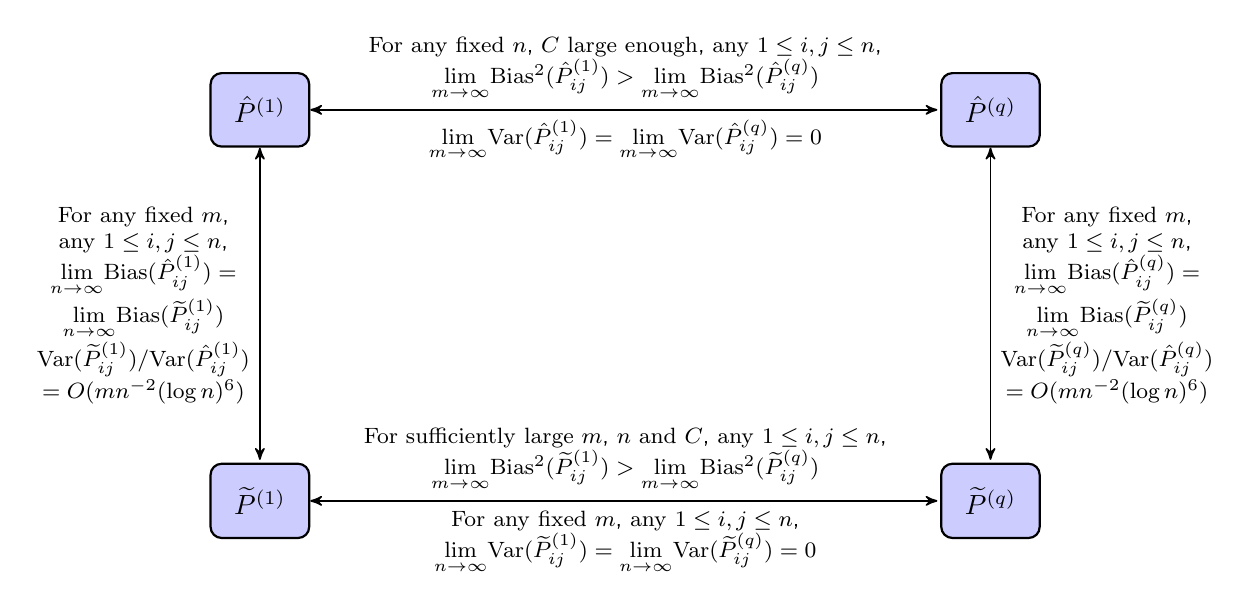
\begin{tikzpicture}[
  font=\sffamily,
  every matrix/.style={ampersand replacement=\&,column sep=2cm,row sep=2cm},
  block/.style={draw,thick,rounded corners,fill=blue!20,inner sep=.3cm},
  process/.style={draw,thick,circle,fill=blue!20},
  sink/.style={source,fill=green!20},
  datastore/.style={draw,very thick,shape=datastore,inner sep=.3cm},
  dots/.style={gray,scale=2},
  to/.style={->,>=stealth',shorten >=1pt,semithick,font=\sffamily\footnotesize},
  tofrom/.style={<->,>=stealth',shorten >=1pt,semithick,font=\sffamily\footnotesize},
  every node/.style={align=center}]

  % Position the nodes using a matrix layout
  \matrix{
    \node[block] (MLE) {$\hat{P}^{(1)}$};
      \& \& \& \& \node[block] (MLqE) {$\hat{P}^{(q)}$};\\
	\\
    \node[block] (XMLE) {$\widetilde{P}^{(1)}$};
      \& \& \& \& \node[block] (XMLqE) {$\widetilde{P}^{(q)}$}; \\
  };

  % Draw the arrows between the nodes and label them.
  \draw[tofrom] (MLE) -- node[midway,above] {$\mathrm{For}$ $\mathrm{any}$ $\mathrm{fixed}$ $n$, $C$ $\mathrm{large}$ $\mathrm{enough}$, $\mathrm{any}$ $1 \le i, j \le n$, \\$\underset{m \to \infty}{\lim} \mathrm{Bias}^2(\hat{P}_{ij}^{(1)}) > \underset{m \to \infty}{\lim} \mathrm{Bias}^2(\hat{P}_{ij}^{(q)})$}
      node[midway,below] {$\underset{m \to \infty}{\lim} \mathrm{Var}(\hat{P}_{ij}^{(1)}) = \underset{m \to \infty}{\lim} \mathrm{Var}(\hat{P}_{ij}^{(q)}) = 0$} (MLqE);
  \draw[tofrom] (MLE) -- node[midway,left] {$\mathrm{For}$ $\mathrm{any}$ $\mathrm{fixed}$ $m$, \\$\mathrm{any}$ $1 \le i, j \le n$, \\$\underset{n \to \infty}{\lim} \mathrm{Bias}(\hat{P}_{ij}^{(1)}) =$\\$ \underset{n \to \infty}{\lim} \mathrm{Bias}(\widetilde{P}_{ij}^{(1)})$\\$\mathrm{Var}(\widetilde{P}_{ij}^{(1)})/\mathrm{Var}(\hat{P}_{ij}^{(1)})$\\$ = O(m n^{-2} (\log n)^6)$} (XMLE);
  \draw[tofrom] (MLqE) -- node[midway,right] {$\mathrm{For}$ $\mathrm{any}$ $\mathrm{fixed}$ $m$, \\$\mathrm{any}$ $1 \le i, j \le n$, \\$\underset{n \to \infty}{\lim} \mathrm{Bias}(\hat{P}_{ij}^{(q)}) = $\\$\underset{n \to \infty}{\lim} \mathrm{Bias}(\widetilde{P}_{ij}^{(q)})$\\$\mathrm{Var}(\widetilde{P}_{ij}^{(q)})/\mathrm{Var}(\hat{P}_{ij}^{(q)})$\\$= O(m n^{-2} (\log n)^{6})$} (XMLqE);
  \draw[tofrom] (XMLE) -- node[midway,above] {$\mathrm{For}$ $\mathrm{sufficiently}$ $\mathrm{ large}$ $m$, $n$ $\mathrm{and}$ $C$, $\mathrm{any}$ $1 \le i, j \le n$, \\$\underset{m \to \infty}{\lim} \mathrm{Bias}^2(\widetilde{P}_{ij}^{(1)}) > \underset{m \to \infty}{\lim} \mathrm{Bias}^2(\widetilde{P}_{ij}^{(q)})$}
      node[midway,below] {$\mathrm{For}$ $\mathrm{any}$ $\mathrm{fixed}$ $m$, $\mathrm{any}$ $1 \le i, j \le n$, \\$\underset{n \to \infty}{\lim} \mathrm{Var}(\widetilde{P}_{ij}^{(1)}) = \underset{n \to \infty}{\lim} \mathrm{Var}(\widetilde{P}_{ij}^{(q)}) = 0$} (XMLqE);
\end{tikzpicture}
\end{center}
\caption{\label{fig:summary}Relationship between four estimators.}
\end{figure}

\RT{The figure of relationship is NOT right.}









\section{Proof}

\subsection{$\hat{P}^{(q)}$ better than $\hat{P}^{(1)}$}

\begin{lemma}
\label{lemma:LqlMLE}
Consider the model $X_1, \cdots, X_m \stackrel{iid}{\sim} \mathrm{Exp}(\theta)$ with $E[X_1] = \theta$. Given any data $x = (x_1, \cdots, x_m)$ such that $x_{(1)} > 0$ and not all $x_i$'s are the same, then $\hat{\theta}_q(x) < \hat{\theta}_1(x)$ for $0 < q < 1$, i.e. ML$q$E \cite{ferrari2010, qin2013maximum} is always less than MLE under exponential distribution no matter how the data is sampled.
\end{lemma}
\begin{proof}
The MLE is
\[
	\hat{\theta}_1(x) = \bar{x}.
\]
And the ML$q$E $\hat{\theta}_q(x)$ solves the equation
\[
	\sum_{i=1}^m e^{-\frac{(1-q)x_i}{\hat{\theta}_q(x)}}(x_i - \hat{\theta}_q(x)) = 0.
\]
Consider the continuous function $g(\theta, x) = \sum_{i=1}^m e^{-\frac{(1-q)x_i}{\theta}}(x_i - \theta)$. 

Let $x_{(1)} \le \cdots \le x_{(l)} \le \bar{x} \le x_{(l+1)} \le \cdots \le x_{(m)}$. Define $s_i = \bar{x} - x_{(i)}$ for $1 \le i \le l$, and $t_{i} = x_{(l+i)} - \bar{x}$ for $1 \le i \le m - l$. Note that $\sum_{i=1}^l s_i = \sum_{i=1}^{m-l} t_i$. Then we have
\begin{align*}
g(\hat{\theta}_1(x), x) & = g(\bar{x}, x) \\
& = \sum_{i=1}^m e^{-\frac{(1-q)x_{(i)}}{\bar{x}}}(x_{(i)} - \bar{x}) \\
& = - \sum_{i=1}^l e^{-\frac{(1-q)x_{(i)}}{\bar{x}}}s_i
+ \sum_{i=1}^{m-l} e^{-\frac{(1-q)x_{(i+l)}}{\bar{x}}}t_i\\
& \le - e^{-(1-q)} \sum_{i=1}^l s_i
+ \sum_{i=1}^{m-l} e^{-\frac{(1-q)x_{(i+l)}}{\bar{x}}}t_i\\
& \le - e^{-(1-q)} \sum_{i=1}^{m-l} t_i
+ \sum_{i=1}^{m-l} e^{-\frac{(1-q)x_{(i+l)}}{\bar{x}}}t_i\\
& \le - \sum_{i=1}^{m-l} e^{-\frac{(1-q)x_{(i+l)}}{\bar{x}}}t_i
+ \sum_{i=1}^{m-l} e^{-\frac{(1-q)x_{(i+l)}}{\bar{x}}}t_i\\
= 0,
\end{align*}
and equality holds if and only if all $x_i$'s are the same, which is excluded by the assumption.
Thus $g(\hat{\theta}_1(x), x) < 0$.

Also we know:
\begin{itemize}
\item $g(\hat{\theta}_q(x), x) = 0$;
\item $\lim_{\theta \rightarrow 0^+}g(\theta, x) = 0$;
\item $g(\theta, x) > 0$ when $\theta < x_{(1)}$;
\end{itemize}
Combined with $g(\hat{\theta}_1(x), x) < 0$, we have $\hat{\theta}_q(x) < \hat{\theta}_1(x)$ for $0 < q < 1$.
\end{proof}



\begin{lemma} [Lemma \ref{lemma:ELqlEMLE}]
For any $0 < q < 1$, there exists $C_0(P_{ij}, \epsilon, q) > 0$ such that under the contaminated model with $C > C_0(P_{ij}, \epsilon, q)$,
\[
	\lim_{m \to \infty} \left| E[\hat{P}^{(q)}_{ij}] - P_{ij} \right| < 
    \lim_{m \to \infty} \left| E[\hat{P}^{(1)}_{ij}] - P_{ij} \right|,
\]
for $1 \le i, j, \le n$ and $i \ne j$.
\end{lemma}
\begin{proof}
For the MLE $\hat{P}^{(1)}_{ij} = \bar{A}_{ij}$,
\[
	E[\hat{P}^{(1)}_{ij}] = E[\bar{A}_{ij}]
    = \frac{1}{m} \sum_{t = 1}^m E[A_{ij}^{(t)}]
    = E[A_{ij}^{(1)}]
    = (1-\epsilon) P_{ij} + \epsilon C_{ij}.
\]
For the ML$q$E $\hat{P}^{(q)}_{ij}$, according to Equation (3.2) in \cite{ferrari2010}, the expectation $E[\hat{P}^{(q)}_{ij}]$, denoted as $\theta$ for simplicity, satisfies
\[
\frac{\epsilon C_{ij}}{(C_{ij}(1-q) + \theta)^2} - \frac{\epsilon}{C_{ij}(1-q) + \theta}
+\frac{(1-\epsilon) P_{ij}}{(P_{ij}(1-q) + \theta)^2} - \frac{(1-\epsilon)}{P_{ij}(1-q) + \theta}
= 0,
\]
i.e.
\[
\frac{\epsilon (\theta - C_{ij}q)}{(C_{ij}(1-q) + \theta)^2} =
\frac{(1-\epsilon) (P_{ij} q - \theta)}{(P_{ij}(1-q) + \theta)^2}.
\]
Thus $\theta - C_{ij} q$ and $\theta - P_{ij} q$ should have different signs. Combined with $C_{ij} > P_{ij}$, we have
\[
q P_{ij} < \theta.
\]
To have a smaller bias in absolute value, we need
\[
|\theta - P_{ij}| < \epsilon (C_{ij} - P_{ij}).
\]
Thus combined with Lemma \ref{lemma:LqlMLE}, we need
\[
q P_{ij} > P_{ij} - \epsilon(C_{ij} - P_{ij}),
\]
i.e.
\[
C_{ij} > P_{ij} + \frac{(1-q) P_{ij}}{\epsilon} = C_0(P_{ij}, \epsilon, q).
\]
\end{proof}



\begin{lemma} [Lemma \ref{lemma:VarMLEandLq0}]
\[
	\lim_{m \to \infty} \mathrm{Var}(\hat{P}^{(1)}_{ij})
    = \lim_{m \to \infty} \mathrm{Var}(\hat{P}^{(q)}_{ij}) = 0,
\]
for $1 \le i, j \le n$.
\end{lemma}
\begin{proof}
Both MLE and ML$q$E follows a central limit theorem, which means their variances goes to 0 as $m \to \infty$.
\end{proof}










\subsection{$\widetilde{P}^{(1)}$ better than $\hat{P}^{(1)}$}


\begin{theorem}
\label{thm:BernsteinMatrix}
(Matrix Bernstein: Subexponential Case). Consider a finite sequence $\{X_k\}$ of
independent, random, self-adjoint matrices with dimension $d$. Assume that
\[
	E[X_k] = 0 \text{\ \ \ and \ \ \ }  E[X_k^p] \preceq \frac{p!}{2} R^{p-2} A_k^2 \text{\ \ for } p = 2,3,4, \dots
\]
Compute the variance parameter
\[
	\sigma^2 := \|\sum_k A_k^2\|.
\]
Then the following chain of inequalities holds for all $t \ge 0$.
\[
	P \left( \lambda_{\max} \left( \sum_k X_k \right) \ge t \right) \le d \cdot \exp \left( \frac{-t^2/2}{\sigma^2 + R t} \right).
\]
\end{theorem}
\textbf{Remark:} Theorem 6.2 in \cite{tropp2012user}.








\begin{theorem}[Theorem 3.3]
\label{thm:P1Diff}
Let $P$ and $C$ be two $n$-by-$n$ symmetric matrices satisfying element-wise conditions $0 < P_{ij} \le C_{ij} \le R$ for some constant $R > 0$. For $0 < \epsilon < 1$, we define $m$ symmetric and hollow matrices as
\[
	A^{(t)} \stackrel{iid}{\sim} (1-\epsilon) \mathrm{Exp}(P) + \epsilon \mathrm{Exp}(C),
\]
for $1 \le t \le m$.
Let $\hat{P}^{(1)}$ be the element-wise MLE based on exponential distribution with $m$ observations.
Define $H_{ij}^{(1)} = E[\hat{P}_{ij}^{(1)}] = (1-\epsilon) P_{ij} + \epsilon C_{ij}$,
then for any constant $c > 0$, there exists another constant $n_0(c)$, independent of $n$, $P$, $C$ and $\epsilon$, such that if $n > n_0$, then for all $\eta$ satisfying $n^{-c} \le \eta \le 1/2$,
\[
	P \left( \| \hat{P}^{(1)} - H^{(1)} \|_2 \le 4 R \sqrt{n \ln(n/\eta)/m}\right) \ge 1 - \eta.
\]
\end{theorem}
\textbf{Remark:} This is the extended version of Theorem 3.1 in \cite{oliveira2009concentration}.

\noindent
\begin{proof}
Let $\{e_i\}_{i=1}^n$ be the canonical basis for $\mathbb{R}^n$. For each $1 \le i, j \le n$, define a corresponding matrix $G_{ij}$:
\[
    G_{ij} \equiv \left\{
    \begin{array}{l l}
        e_i e_j^T + e_j e_i^T, \quad & i \ne j;\\
        e_i e_i^T, \quad & i = j.
    \end{array}
    \right.
\]
Thus
\[
\hat{P}^{(1)} = \sum_{1 \le i < j \le n} \hat{P}^{(1)}_{ij} G_{ij} = \frac{1}{m}\sum_{t=1}^m \sum_{1 \le i < j \le n} A^{(t)}_{ij} G_{ij}
\]
and
\[
H^{(1)} = \sum_{1 \le i < j \le n} H^{(1)}_{ij} G_{ij}.
\]
Then we have $\hat{P}^{(1)} - H^{(1)} = \frac{1}{m} \sum_{1 \le t \le m, 1 \le i < j \le n} X_{ij}^{(t)}$, where $X_{ij}^{(t)} \equiv \left( A^{(t)}_{ij} - H^{(1)}_{ij} \right) G_{ij}$ for $1 \le t \le m$ and $1 \le i < j \le n$.

First bound the $k$-th moment of $X_{ij}$ for $1 \le i < j \le n$ as following:
\begin{align*}
	E[(A^{(t)}_{ij} - H^{(1)}_{ij})^k]
    \le & (1-\epsilon) \cdot \exp(-H_{ij}/P_{ij}) P_{ij}^k \Gamma(1+k, -H_{ij}/P_{ij}) \\
    & + \epsilon \cdot \exp(-H_{ij}/C_{ij}) C_{ij}^k \Gamma(1+k, -H_{ij}/C_{ij}) \\
    \le & \left( (1-\epsilon) \cdot \exp(-H_{ij}/P_{ij}) P_{ij}^k + \epsilon \cdot \exp(-H_{ij}/C_{ij}) C_{ij}^k \right) k! \\
    \le & \left( (1-\epsilon) \cdot P_{ij}^k + \epsilon \cdot C_{ij}^k \right) k! \\
    \le & R^k k!,
    \stepcounter{equation}\tag{\theequation}\label{eqn:expectpdiffqpowerkL1}
\end{align*}

Combined with
\[
    G_{ij}^k \equiv \left\{
    \begin{array}{l l}
        e_i e_i^T + e_j e_j^T, \quad & $k$ \text{ is even};\\
        e_i e_j^T + e_j e_i^T, \quad & $k$ \text{ is odd},
    \end{array}
    \right.
\]
thus we have
\begin{enumerate}
\item When $k$ is even,
\[
E[(X_{ij}^{(t)})^k] = E[(A^{(t)}_{ij} - H^{(1)}_{ij})^k] G_{ij}^2 \preceq k! R^k G_{ij}^2;
\]
\item When $k$ is odd,
\[
E[(X_{ij}^{(t)})^k] = E[(A^{(t)}_{ij} - H^{(1)}_{ij})^k] G_{ij} \preceq k! R^k G_{ij}^2.
\]
\end{enumerate}
So
\[
E[(X_{ij}^{(t)})^k] \preceq k! R^k G_{ij}^2.
\]
Let
\[
	\sigma^2 := \left\| \sum_{1 \le t \le m, 1 \le i < j \le n} (\sqrt{2} R G_{ij})^2 \right\|_2 = 2 R^2 m \| (n - 1) I \|_2 = 2 R^2 m (n - 1).
\]
Notice that random matrices $X_{ij}^{(t)}$ are independent, self-adjoint and have mean zero, apply Theorem \ref{thm:BernsteinMatrix} we have
\begin{align*}
	P \left( \lambda_{\max}(\hat{P}^{(1)} - H^{(1)}) \ge t \right)
	& = P \left( \lambda_{\max}(\frac{1}{m} \sum_{1 \le t \le m, 1 \le i < j \le n} X_{ij}^{(t)}) \ge t \right) \\
	& = P \left( \lambda_{\max}(\sum_{1 \le t \le m, 1 \le i < j \le n} X_{ij}^{(t)}) \ge m t \right) \\
	& \le n \exp \left( - \frac{(m t)^2/2}{\sigma^2 + R m t} \right) \\
	& \le n \exp \left( - \frac{m t^2/2}{2 R^2 n + R t} \right).
\end{align*}

Now consider $Y_{ij}^{(t)} \equiv \left( H_{ij}^{(1)} - A_{ij}^{(t)} \right) G_{ij}$, for $1 \le t \le m$ and $1 \le i < j \le n$. Then we have $H^{(1)} - \hat{P}^{(1)} = \frac{1}{m} \sum_{1 \le t \le m, 1 \le i < j \le n} Y_{ij}^{(t)}$.
Since
\[
	E[(H^{(1)} - \hat{P}^{(1)})^k]
    = (-1)^k E[(\hat{P}^{(1)} - H^{(1)})^k],
\]
\begin{enumerate}
\item When $k$ is even,
\[
E[(Y_{ij}^{(t)})^k] = E[(\hat{P}^{(1)} - H^{(1)})^k] G_{ij}^2 \preceq k! R^k G_{ij}^2;
\]
\item When $k$ is odd,
\[
E[Y_{ij}^k] = - E[(\hat{P}^{(1)} - H^{(1)})^k] G_{ij} \preceq k! R^k G_{ij}^2.
\]
\end{enumerate}
Thus by similar arguments,
\begin{align*}
	P \left( \lambda_{\min}(\hat{P}^{(1)} - H^{(1)}) \le -t \right) &
    = P \left( \lambda_{\max}(H^{(1)} - \hat{P}^{(1)}) \ge t \right) \\
    & \le n \exp \left( - \frac{m t^2/2}{2 R^2 n + R t} \right).
\end{align*}
Therefore we have
\[
	P \left( \| \hat{P}^{(1)} - H^{(1)} \|_2 \ge t \right)
    \le n \exp \left( - \frac{m t^2/2}{2 R^2 n + R t} \right).
\]

Now let $c > 0$ be given and assume $n^{-c} \le \eta \le 1/2$. Then there exists a $n_0(c)$ independent of $n$, $P$, $C$ and $\epsilon$ such that whenever $n > n_0(c)$,
\[
	t =  4 R \sqrt{n \ln(n/\eta)/m} \le 6 R n.
\]

Plugging this $t$ into the equation above, we get
\[
	P(\| \hat{P}^{(1)} - H^{(1)} \|_2 \ge 4 R \sqrt{n \ln(n/\eta)/m})
    \le n \exp\left(-\frac{t^2}{16 R^2 n}\right) = \eta.
\]
\end{proof}

Define $H^{(1)} = E[\hat{P}^{(1)}] = (1-\epsilon) P + \epsilon C$, where $P = X X^T$, $X \in \mathbb{R}^{n \times d}$, $C = Y Y^T$, $Y \in \mathbb{R}^{n\times d'}$.
Let $d^{(1)} = \mathrm{rank}(H^{(1)})$ be the dimension in which we are going to embed $\hat{P}^{(1)}$. Then we can define $H^{(1)} = Z Z^T$ where $Z \in \mathbb{R}^{n \times d^{(1)}}$.
Since $H^{(1)} = [\sqrt{1-\epsilon} X, \sqrt{\epsilon} Y] [\sqrt{1-\epsilon} X, \sqrt{\epsilon} Y]^T$, we have $d^{(1)} \le d+d'$.


For simplicity, from now on, we will use $\hat{P}$ to represent $\hat{P}^{(1)}$, use $H$ to represent $H^{(1)}$ and use $k$ to represent the dimension $d^{(1)}$ we are going to embed. Assume $H = U S U^T = Z Z^T$, where $Z = [Z_1, \cdots, Z_n]^T$ is a $n$-by-$k$ matrix. Then our estimate for $Z$ up to rotation is $\hat{Z} = \hat{U} \hat{S}^{1/2}$, where $\hat{U} \hat{S} \hat{U}^T$ is the rank-$k$ spectral decomposition of $|\hat{P}| = (\hat{P}^T \hat{P})^{1/2}$.

Furthermore, we assume that the second moment matrix $E[Z_1 Z_1^T]$ is rank $k$ and has distinct eigenvalues $\lambda_i(E[Z_1 Z_1^T])$. In particular, we assume that there exists $\delta > 0$ such that
\[
	\delta < \min \left( \min_{i \ne j} |\lambda_i(E[Z_1 Z_1^T]) - \lambda_j(E[Z_1 Z_1^T])|, \lambda_k(E[Z_1 Z_1^T]) \right)
\]

\begin{lemma}
\label{lemma:eigSShatL1}
Under the above assumptions, $\lambda_i(H) = \Theta(n)$ with high probability when $i \le k$, i.e. the largest $k$ eigenvalues of $H$ is of order $n$. Moreover, we have $\| S \|_2 = \Theta(n)$ and $\| \hat{S} \|_2 = \Theta(n)$ with high probability.
\end{lemma}
\textbf{Remark:} This is a extended version of Proposition 4.3 in \cite{sussman2014consistent}.

\noindent
\begin{proof}
Note that $\lambda_i(H) = \lambda_i(Z Z^T) = \lambda_i(Z^T Z)$ when $i \le k$. Since each entry of $Z^T Z$ is a sum of $n$ independent random variables each in $[0, R]$, i.e. $(Z^T Z)_{ij} = \sum_{l = 1}^n Z_{li} Z_{lj}$. By Hoeffding's inequality, for each entry we have
\[
P(|(Z^T Z - n E[Z_1 Z_1^T])_{ij}| \ge R \sqrt{n\log{n}}) \le \frac{2}{n^2}.
\]
By the union bound, we have
\[
P(\|(Z^T Z - n E[Z_1 Z_1^T])_{ij}\|_F \ge k R \sqrt{n\log{n}}) \le \frac{2 k^2}{n^2}.
\]
Then by Weyl's Theorem \cite{horn2012matrix}, we have
\[
|\lambda_i(H) - n \lambda_i(Z_1 Z_1^T)| \le \|Z^T Z - n E[Z_1 Z_1^T]\|_2 \le k R \sqrt{n\log{n}}
\]
with probability at least $1 - \frac{2 k^2}{n^2}$.
Thus $\lambda_i(H) = S_{ii} = \Theta(n)$ with probability at least $1 - \frac{2 k^2}{n^2}$ when $i \le k$.

Moreover,
\[
\| H \|_2 - \|H - \hat{P}\|_2 \le \|\hat{S}\|_2 \le \|\hat{P} - H\|_2 + \|H\|_2.
\]
Combined with Theorem \ref{thm:P1Diff}, with high probability we have $\|\hat{S}\|_2 = \Theta(n)$.
\end{proof}


\begin{lemma}
\label{lemma:AlmostOrthogonalL1}
Let $W_1 \Sigma W_2^T$ be the singular value decomposition of $U^T \hat{U}$. Then for sufficiently large $n$, 
\[
	\| U^T \hat{U} - W_1 W_2^T \|_F = O(m^{-1} n^{-1} \log n)
\]
with high probability.
\end{lemma}
\begin{proof}
Let $\sigma_1, \cdots, \sigma_d$ denote the singular values of $U^T \hat{U}$. Then $\sigma_i = \cos(\theta_i)$ where the $\theta_i$ are the principal angles between the subspaces spanned by $\hat{U}$ and $U$. Furthermore, by the Davis-Kahan $\sin(\Theta)$ theorem \cite{davis1970rotation}, combined with Theorem \ref{thm:P1Diff} and Lemma \ref{lemma:eigSShatL1},
\begin{equation}
\label{eqn:uhat2u2diffL1}
	\|\hat{U} \hat{U}^T - U U^T\|_2 = \max_i |\sin(\theta_i)|
    \le \frac{\|\hat{P} - H\|_2}{\lambda_k(H)}
    \le \frac{C \sqrt{n \log n/m}}{n} = O(m^{-1/2} n^{-1/2} \sqrt{\log n})
\end{equation}
for sufficiently large $n$. Here $\lambda_k(H)$ denotes the $k$-th largest eigenvalue of $H$.\\
We thus have
\begin{align*}
	\| U^T \hat{U} - W_1 W_2^T \|_F
    & = \| \Sigma - I \|_F
    = \sqrt{\sum_{i=1}^k (1-\sigma_i)^2} \\
    & \le \sum_{i=1}^k (1-\sigma_i) \le \sum_{i=1}^k (1-\sigma_i^2) \\
    & = \sum_{i=1}^k \sin^2(\theta_i)
    \le k \|\hat{U} \hat{U}^T - U U^T\|_2^2 \\
    & = O(m^{-1} n^{-1} \log n).
\end{align*}
\end{proof}

We will denote the orthogonal matrix $W_1 W_2^T$ by $W^*$.

\begin{lemma}
\label{lemma:exchangeL1}
For sufficiently large $n$,
\[
	\| W^* \hat{S} - S W^* \|_F = O(m^{-1/2} \log n),
\]
\[
	\|W^* \hat{S}^{1/2} - S^{1/2} W^* \|_F = O(m^{-1/2} n^{-1/2} \log n)
\]
and
\[
	\| W^* \hat{S}^{-1/2} - S^{-1/2} W^* \|_F = O(m^{-1/2} n^{-3/2} \log n)
\]
with high probability.
\end{lemma}
\begin{proof}
By Proposition 2.1 in \cite{rohe2011spectral} and Equation (\ref{eqn:uhat2u2diffL1}), we have for some orthogonal matrix $W$,
\[
\|\hat{U} - U W\|_F^2 \le \frac{2 \|\hat{U} \hat{U}^T - U U^T\|_F^2}{\delta^2} = O(m^{-1/2} n^{-1/2} \sqrt{\log n}).
\]
\RT{Not right here, I am using the result for spectral norm as frobenius norm.}
Let $Q = \hat{U} - U U^T \hat{U}$. And $Q$ is the residual after projecting $\hat{U}$ orthogonally onto the column space of $U$, we have
\begin{equation}
\label{eqn:QFnormL1}
\| Q \|_F = \| \hat{U} - U U^T \hat{U} \|_F \le \| \hat{U} - U T \|_F = O(m^{-1/2} n^{-1/2} \sqrt{\log n}).
\end{equation}
for all $k \times k$ matrices $T$. 

Then
\begin{align*}
	W^* \hat{S} = & (W^* - U^T \hat{U}) \hat{S} + U^T \hat{U} \hat{S}
    = (W^* - U^T \hat{U}) \hat{S} + U^T \hat{P} \hat{U} \\
    = & (W^* - U^T \hat{U}) \hat{S} + U^T (\hat{P} - H) \hat{U} + U^T H \hat{U} \\
    = & (W^* - U^T \hat{U}) \hat{S} + U^T (\hat{P} - H) Q + U^T (\hat{P} - H) U U^T \hat{U} + U^T H \hat{U} \\
    = & (W^* - U^T \hat{U}) \hat{S} + U^T (\hat{P} - H) Q + U^T (\hat{P} - H) U U^T \hat{U} + S U^T \hat{U}.
\end{align*}
Combined with Theorem \ref{thm:P1Diff}, Lemma \ref{lemma:eigSShatL1}, Lemma \ref{lemma:AlmostOrthogonalL1}, we have
\begin{align*}
	& \| W^* \hat{S} - S W^* \|_F \\
    = & \| (W^* - U^T \hat{U}) \hat{S} + U^T (\hat{P} - H) Q + U^T (\hat{P} - H) U U^T \hat{U} + S (U^T \hat{U} - W^*)\|_F \\
    \le & \| W^* - U^T \hat{U} \|_F (\| \hat{S} \|_2 + \| S \|_2) + \| U^T \|_F \| \hat{P} - H\|_2 \| Q \|_F + \| U^T (\hat{P} - H) U \|_F \\
    \le & O(m^{-1} \log n) + O(m^{-1/2} \log n) + \| U^T (\hat{P} - H) U \|_F
\end{align*}
with high probability. And we know $U^T (\hat{P} - H) U$ is a $k \times k$ matrix with $ij$-th entry to be
\[
	u_i^T (\hat{P} - H) u_j
    = \sum_{s=1}^n \sum_{t=1}^n (\hat{P}_{st} - H_{st}) u_{is} u_{jt}
    = 2 \sum_{s<t} (\hat{P}_{st} - H_{st}) u_{is} u_{jt}
\]
where $u_i$ and $u_j$ are the $i$-th and $j$-th columns of $U$. Thus, conditioned on $H$, $U$ is fixed and $u_i^T (\hat{P} - H) u_j$ is a sum of independent mean 0 random variables.


By Equation (\ref{eqn:expectpdiffqpowerkL1}), we have
\begin{align*}
	& E\left[\left((A^{(t')}_{st} - H_{st}) u_{is} u_{jt}\right)^k\right] \\
    \le & k! R^k u_{is}^k u_{jt}^k \\
    \le & \frac{k!}{2} R^{k-2} (\sqrt{2} u_{is} u_{jt} R)^2.
\end{align*}
Also we have
\[
	\sigma^2 := |\sum_{t', s<t} 2 R^2 u_{is}^2 u_{jt}^2| \le m R^2,
\]
then by Theorem \ref{thm:BernsteinMatrix}, we have
\[
	P \left( \left| 2 \sum_{s<t} (\hat{P}_{st} - H_{st}) u_{is} u_{jt} \right| \ge t \right)
    \le \exp \left( \frac{-m t^2/8}{R^2 + R t /2} \right).
\]
Let $t = m^{-1/2} \log n$, we have
\[
P \left( \left| 2 \sum_{s<t} (\hat{P}_{st} - H_{st}) u_{is} u_{jt} \right| \ge m^{-1} \log n \right)
    \le n^{-c},
\]
where $c = 1/(8R)$.
Thus each entry of $U^T(\hat{P} - H)U$ is of order $O(m^{-1} \log n)$ with high probability and
\begin{equation}
\label{eqn:uPhatdiffHuL1}
	\|U^T(\hat{P} - H)U\|_F = O(m^{-1} \log n)
\end{equation}
with high probability.
Hence
\[
	\| W^* \hat{S} - S W^* \|_F = O(m^{-1/2} \log n)
\]
with high probability.
Also, since
\[
	W_{ij}^* (\lambda_j^{1/2}(\hat{P}) - \lambda_i^{1/2}(H)) = W_{ij}^* \frac{\lambda_j(\hat{P}) - \lambda_i(H)}{\lambda_j^{1/2}(\hat{P}) + \lambda_i^{1/2}(H)}
\]
and the eigenvalues $\lambda_j^{1/2}(\hat{P})$ and $\lambda_i^{1/2}(H)$ are both of order $\Theta(\sqrt{n})$, we have
\[
	\| W^* \hat{S}^{1/2} - S^{1/2} W^* \|_F = O(m^{-1/2} n^{-1/2} \log n).
\]
Similarly, since
\[
	W_{ij}^* (\lambda_j^{-1/2}(\hat{P}) - \lambda_i^{-1/2}(H)) = W_{ij}^* \frac{\lambda_i(H) - \lambda_j(\hat{P})}{(\lambda_j^{-1/2}(\hat{P}) + \lambda_i^{-1/2}(H))\lambda_j(\hat{P}) \lambda_i(H)}
\]
and the eigenvalues $\lambda_j(\hat{P})$ and $\lambda_i(H)$ are both of order $\Theta(n)$, we have
\[
	\| W^* \hat{S}^{-1/2} - S^{-1/2} W^* \|_F = O(m^{-1/2} n^{-3/2} \log n).
\]
\end{proof}



\begin{lemma}
\label{lemma:XhatDiffXWexpressionL1}
There exists a rotation matrix $W$ such that for sufficiently large $n$,
\[
	\|\hat{Z} - Z W\|_F = \| (\hat{P} - H) U S^{-1/2} \|_F + O(m^{-1/2} n^{-1/2} (\log n)^{3/2})
\]
with high probability.
\end{lemma}
\begin{proof}
Let $Q_1 = U U^T \hat{U} - U W^*$, $Q_2 = W^* \hat{S}^{1/2} - S^{1/2} W^*$ and $Q_3 = \hat{U} - U W^* = \hat{U} - U U^T \hat{U} + Q_1 = Q + Q_1$. Then since $U U^T P = P$ and $\hat{U} \hat{S}^{1/2} = \hat{P} \hat{U} \hat{S}^{-1/2}$,
\begin{align*}
	\hat{Z} - U S^{1/2} W^*
    = & \hat{U} \hat{S}^{1/2} - U W^* \hat{S}^{1/2} + U(W^* \hat{S}^{1/2} - S^{1/2} W^*) \\
    = & (\hat{U} - U U^T \hat{U}) \hat{S}^{1/2} + Q_1 \hat{S}^{1/2} + U Q_2 \\
    = & (\hat{P} - H) \hat{U} \hat{S}^{-1/2} - U U^T(\hat{P} - H)\hat{U}\hat{S}^{-1/2} + Q_1 \hat{S}^{1/2} + U Q_2 \\
    = & (\hat{P} - H) U W^* \hat{S}^{-1/2} - U U^T(\hat{P} - H)U W^*\hat{S}^{-1/2} \\
    & + (I - U U^T)(\hat{P} - H) Q_3 \hat{S}^{-1/2} + Q_1 \hat{S}^{1/2} + U Q_2.
\end{align*}
By Lemma \ref{lemma:AlmostOrthogonalL1},
\[
	\|Q_1\|_F \le \| U\|_F \| U^T \hat{U} - W^* \|_F = O(m^{-1} n^{-1} \log n).
\]
By Lemma \ref{lemma:exchangeL1},
\[
	\|Q_2\|_F = O(m^{-1/2} n^{-1/2} \log n).
\]
By Equation (\ref{eqn:QFnormL1}),
\[
	\|Q_3\|_F \le \|Q\|_F + \|Q_1\|_F = O(m^{-1/2} n^{-1/2} (\log n)^{1/2}).
\]
By Equation (\ref{eqn:uPhatdiffHuL1}),
\[
	\| U U^T(\hat{P} - H)U W^*\hat{S}^{-1/2} \|_F
    \le \| U^T(\hat{P} - H)U \|_F \| \hat{S}^{-1/2} \|_2
    = O(m^{-1} n^{-1/2} \log n).
\]
By Lemma \ref{lemma:exchangeL1},
\[
	\| W^* \hat{S}^{-1/2} - S^{-1/2} W^* \|_F = O(m^{-1/2} n^{-3/2} \log n).
\]
Therefore,
\begin{align*}
	& \| \hat{Z} - U S^{1/2} W^* \|_F \\
    = & \| (\hat{P} - H) U W^* \hat{S}^{-1/2} \|_F + O(m^{-1} n^{-1/2} \log n)
    + \|I - U U^T \|_2 \| \hat{P} - H \|_2 O(m^{-1/2} n^{-1} (\log n)^{1/2}) \\
    & + O(m^{-1} n^{-1/2} \log n) + O(m^{-1/2} n^{-1/2} \log n)\\
    = & \| (\hat{P} - H) U W^* \hat{S}^{-1/2} \|_F + O(m^{-1/2} n^{-1/2} \log n) \\
    \le & \| (\hat{P} - H) U S^{-1/2} W^* \|_F + \|(\hat{P} - H) U (W^* \hat{S}^{-1/2} - S^{-1/2} W^*) \|_F + O(m^{-1/2} n^{-1/2} \log n) \\
    = & \| (\hat{P} - H) U S^{-1/2}\|_F + O(m^{-1} n^{-1} (\log n)^{3/2}) + O(m^{-1/2} n^{-1/2} (\log n)^{3/2}) \\
    = & \| (\hat{P} - H) U S^{-1/2}\|_F + O(m^{-1/2} n^{-1/2} (\log n)^{3/2}).
\end{align*}
\RT{$\|I - U U^T\|_2 = O(1)$}
Note that $Z = U S^{1/2} W$ for some orthogonal matrix $W$. As $W^*$ is also orthogonal, therefore $Z \tilde{W} = U S^{1/2} W^*$ for some orthogonal $\tilde{W}$, which completes the proof.
\end{proof}




\begin{theorem}
\label{thm:XhatDiffXWL1}
There exists a rotation matrix $W$ such that for sufficiently large $n$,
\[
	\max_i \| \hat{Z}_i - W Z_i \|_2 = O(m^{-1/2} n^{-1/2} (\log n)^{3/2})
\]
with high probability.
\end{theorem}
\begin{proof}
By Lemma \ref{lemma:XhatDiffXWexpressionL1}, we have
\[
	\|\hat{Z} - Z W\|_F = \| (\hat{P} - H) U S^{-1/2} \|_F + O(m^{-1/2} n^{-1/2} (\log n)^{3/2})
\]
and similarly we could have the bound for each column vector
\begin{align*}
	\max_i \| \hat{Z}_i - W Z_i \|_2
    \le & \frac{1}{\lambda_k^{1/2}(H)} \max_i \| ((\hat{P} - H) U)_i \|_2 + O(m^{-1/2} n^{-1/2} (\log n)^{3/2}) \\
    \le & \frac{k^{1/2}}{\lambda_k^{1/2}(H)} \max_j \| (\hat{P} - H) u_j \|_{\infty} + O(m^{-1/2} n^{-1/2} (\log n)^{3/2})
\end{align*}
where $((\hat{P} - H) U)_i$ represents the $i$-th row of $(\hat{P} - H) U$ and $u_j$ denotes the $j$-th column of $U$. Now given $i$ and $j$, the $i$-th element of the vector $(\hat{P} - H) u_j$ is of the form
\[
	\sum_{s=1}^n (\hat{P}_{is} - H_{is}) u_{js} = \sum_{s \ne i} (\hat{P}_{is} - H_{is}) u_{js}.
\]
Thus, conditioned on $H$, the $i$-th element of the vector $(\hat{P} - H) u_j$ is a sum of independent mean 0 random variables.
By Equation (\ref{eqn:expectpdiffqpowerkL1}), we have
\begin{align*}
	& E\left[\left((A^{(t)}_{is} - H_{is}) u_{js}\right)^k\right] \\ 
    \le & k! R^k u_{js}^k \\
    \le & \frac{k!}{2} R^{k-2} (\sqrt{2} R u_{js})^2.
\end{align*}
Also we have
\[
	\sigma^2 := |\sum_{t, s \ne i} 2 R^2 u_{js}^2| \le 2 R^2 m,
\]
then by Theorem \ref{thm:BernsteinMatrix}, we have
\[
	P \left( \left| \sum_{s \ne i} (\hat{P}_{is} - H_{is}) u_{js} \right| \ge t \right)
    \le \exp \left( \frac{-m t^2/2}{2 R^2 + R t} \right),
\]
i.e. it is of order $O(m^{-1} \log n)$ with high probability.
Taking the union bound over all $i$ and $j$, with high probability we have,
\begin{align*}
	\max_i \| \hat{Z}_i - W Z_i \|_2
    & \le \frac{C k^{1/2}}{\lambda_k^{1/2}(H)} m^{-1} (\log n)^{3/2} + O(m^{-1/2} n^{-1/2} (\log n)^{3/2}) \\
    & = O(m^{-1/2} n^{-1/2} (\log n)^{3/2}).
\end{align*}
\end{proof}




\begin{lemma}
\label{lemma:1stMomentPhatDiffL1}
$\left|  \hat{Z}_i^T \hat{Z}_j - Z_i^T Z_j \right| = O(m^{-1/2} n^{-1} (\log n)^{3})$ with high probability.
\end{lemma}
\begin{proof}
Let $W$ be the rotation matrix in Theorem \ref{thm:XhatDiffXWL1}, then
\begin{align*}
	\left|  \hat{Z}_i^T \hat{Z}_j - Z_i^T Z_j \right|
    = & \left| \hat{Z}_i^T \hat{Z}_j - \hat{Z}_i^T W Z_j + \hat{Z}_i^T W Z_j - (W Z_i)^T W Z_j \right| \\
    \le & \left| \hat{Z}_i^T (\hat{Z}_j - W Z_j) + (\hat{Z}_i^T - (W Z_i)^T) W Z_j \right| \\
    \le & \|\hat{Z}_i\|_2 \|\hat{Z}_j - W Z_j\|_2 + \|Z_j\|_2 \|\hat{Z}_i^T - (W Z_i)^T\|_2.
\end{align*}
Since $\|Z_i\|_2^2 = Z_i^T Z_i = H^{(1)}_{ii} =  E[\hat{P}^{(1)}_{ii}] = (1-\epsilon) P_{ij} + \epsilon C_{ij} \le R$, we have $\|Z_i\|_2 = O(1)$.
Combined with Theorem \ref{thm:XhatDiffXWL1},
\begin{align*}
    \left|  \hat{Z}_i^T \hat{Z}_j - Z_i^T Z_j \right|
    = & (\|\hat{Z}_i\|_2 + \|Z_j\|_2) O(n^{-1/2} (\log n)^{3/2}) \\
    \le & (\|\hat{Z}_i - W Z_i\|_2 + \|W Z_i\|_2 + \|Z_j\|_2) O(m^{-1/2} n^{-1/2} (\log n)^{3/2}) \\
    = & O(m^{-1/2} n^{-1} (\log n)^{3})
\end{align*}
with high probability.
\end{proof}




\begin{corollary}
\label{cor:L1Consistent}
For fixed $m$, the estimator based on ASE of MLE has the same entry-wise asymptotic bias as MLE, i.e.
\[
	\lim_{n \to \infty} \mathrm{Bias}(\widetilde{P}_{ij}^{(1)}) = \lim_{n \to \infty} E[\widetilde{P}_{ij}^{(1)}] - P_{ij} = \lim_{n \to \infty} E[\hat{P}^{(1)}_{ij}] - P_{ij}
    = \lim_{n \to \infty} \mathrm{Bias}(\hat{P}_{ij}^{(1)}).
\]
\end{corollary}
\begin{proof}
Direct result from Lemma \ref{lemma:1stMomentPhatDiffL1} by noticing
\[
	\lim_{n \to \infty} E[\widetilde{P}_{ij}^{(1)}] = \lim_{n \to \infty} E[\hat{P}^{(1)}_{ij}].
\]
\end{proof}


Define $(\hat{Z}_i^T \hat{Z}_j)_{\mathrm{tr}}$, our estimator for $P_{ij}$, to be a projection of $\hat{Z}_i^T \hat{Z}_j$ onto $[0, \max(\hat{P}_{ij}, R)]$.

\begin{theorem}
\label{thm:VarASEL1}
Assuming that $m = o(n^{2\epsilon})$, then $\mathrm{Var}((\hat{Z}_i^T \hat{Z}_j)_{\mathrm{tr}}) = O(m^{-1} n^{-2(1-\epsilon)})$.
\end{theorem}
\begin{proof}
By Lemma \ref{lemma:1stMomentPhatDiffL1},
\begin{align*}
	\mathrm{Var}((\hat{Z}_i^T \hat{Z}_j)_{\mathrm{tr}})
    = & E[((\hat{Z}_i^T \hat{Z}_j)_{\mathrm{tr}} - E[(\hat{Z}_i^T \hat{Z}_j)_{\mathrm{tr}}])^2] \\
    = & E[((\hat{Z}_i^T \hat{Z}_j)_{\mathrm{tr}} - Z_i^T Z_j + Z_i^T Z_j - E[(\hat{Z}_i^T \hat{Z}_j)_{\mathrm{tr}}])^2] \\
    = & E[((\hat{Z}_i^T \hat{Z}_j)_{\mathrm{tr}} - Z_i^T Z_j)^2] + E[(Z_i^T Z_j - E[(\hat{Z}_i^T \hat{Z}_j)_{\mathrm{tr}}])^2] \\ 
    & + 2E[((\hat{Z}_i^T \hat{Z}_j)_{\mathrm{tr}} - Z_i^T Z_j)(Z_i^T Z_j - E[(\hat{Z}_i^T \hat{Z}_j)_{\mathrm{tr}}])] \\
    \le & E[((\hat{Z}_i^T \hat{Z}_j)_{\mathrm{tr}} - Z_i^T Z_j)^2] + E[(Z_i^T Z_j - E[(\hat{Z}_i^T \hat{Z}_j)_{\mathrm{tr}}])^2] \\ 
    & + 2\sqrt{E[((\hat{Z}_i^T \hat{Z}_j)_{\mathrm{tr}} - Z_i^T Z_j)^2] E[(Z_i^T Z_j - E[(\hat{Z}_i^T \hat{Z}_j)_{\mathrm{tr}}])^2]} \\
    \le & 4 E[((\hat{Z}_i^T \hat{Z}_j)_{\mathrm{tr}} - Z_i^T Z_j)^2]
\end{align*}
Fix some $a > 0$, we have
\begin{align*}
	& E[((\hat{Z}_i^T \hat{Z}_j)_{\mathrm{tr}} - Z_i^T Z_j)^2] \\
	= & E[((\hat{Z}_i^T \hat{Z}_j)_{\mathrm{tr}} - Z_i^T Z_j)^2 \mathbb{I}\{\hat{P}_{ij} \le a\}]
	+ E[((\hat{Z}_i^T \hat{Z}_j)_{\mathrm{tr}} - Z_i^T Z_j)^2 \mathbb{I}\{\hat{P}_{ij} > a\}]
\end{align*}
For the first term, we have
\begin{align*}
	& E[((\hat{Z}_i^T \hat{Z}_j)_{\mathrm{tr}} - Z_i^T Z_j)^2 \mathbb{I}\{\hat{P}_{ij} \le a\}] \\
	\le & E[((\hat{Z}_i^T \hat{Z}_j)_{\mathrm{tr}} - Z_i^T Z_j)^2 \mathbb{I}\{\hat{P}_{ij} \le a\} \mathbb{I}\{\mathrm{Lemma 4.11 holds}\}] (1 - \frac{1}{n^2}) \\
	& + E[((\hat{Z}_i^T \hat{Z}_j)_{\mathrm{tr}} - Z_i^T Z_j)^2 \mathbb{I}\{\hat{P}_{ij} \le a\} \mathbb{I}\{\mathrm{Lemma 4.11 does not hold}\}] \frac{1}{n^2} \\
	\le & O(m^{-1} n^{-2(1-\epsilon)}) (1 - \frac{1}{n^2}) + \frac{1}{n^2} 2 E[((\hat{Z}_i^T \hat{Z}_j)_{\mathrm{tr}} - \hat{P}_{ij})^2 \mathbb{I}\{\hat{P}_{ij} \le a\}] \\
	& + \frac{1}{n^2} 2 E[(\hat{P}_{ij} - Z_i^T Z_j)^2 \mathbb{I}\{\hat{P}_{ij} \le a\}] \\
	\le & O(m^{-1} n^{-2(1-\epsilon)}) + \frac{2}{n^2} E[\hat{P}_{ij}^2 \mathbb{I}\{\hat{P}_{ij} \le a\}] + \frac{2}{n^2} E[(\hat{P}_{ij} + M)^2 \mathbb{I}\{\hat{P}_{ij} \le a\}] \\
	\le & O(m^{-1} n^{-2(1-\epsilon)}) + \frac{2 a^2}{n^2} + \frac{2 (a+R)^2}{n^2} \\
	\le & O(m^{-1} n^{-2(1-\epsilon)}) + \frac{4}{n^2} (a + R)^2
\end{align*}
For the second term, we have
\begin{align*}
	& E[((\hat{Z}_i^T \hat{Z}_j)_{\mathrm{tr}} - Z_i^T Z_j)^2 \mathbb{I}\{\hat{P}_{ij} > a\}] \\
	\le & 2 E[((\hat{Z}_i^T \hat{Z}_j)_{\mathrm{tr}} - \hat{P}_{ij})^2 \mathbb{I}\{\hat{P}_{ij} > a\}] + 2 E[(\hat{P}_{ij} - Z_i^T Z_j)^2 \mathbb{I}\{\hat{P}_{ij} > a\}] \\
	\le & 2 E[\hat{P}_{ij}^2 \mathbb{I}\{\hat{P}_{ij} > a\}] + 2 E[(\hat{P}_{ij} + M)^2 \mathbb{I}\{\hat{P}_{ij} > a\}] \\
	\le & 2 E[A^{(t)2}_{ij} \mathbb{I}\{A^{(t)}_{ij} > a\}] + 2 E[(A^{(t)}_{ij} + M)^2 \mathbb{I}\{A^{(t)}_{ij} > a\}] \\
	\le & 2 e^{-a/R} \left( 2a^2 + 7R^2 + 6a R \right) \\
	\le & 4 e^{-a/R} (a + 3R)^2
\end{align*}
Thus,
\[
	\mathrm{Var}((\hat{Z}_i^T \hat{Z}_j)_{\mathrm{tr}}) \le
	O(m^{-1} n^{-2(1-\epsilon)}) + 16 (a+3R)^2 (\frac{1}{n^2} + e^{-a/R}).
\]
Let $a = m^{-1/2} n^{\epsilon}$ for any $\epsilon > 0$, combined with the assumption $m = o(n^{2\epsilon})$, we have
\begin{align*}
	\mathrm{Var}((\hat{Z}_i^T \hat{Z}_j)_{\mathrm{tr}})
	\le & 	O(m^{-1} n^{-2} (\log n)^6) + 16 m^{-1} n^{2\epsilon} (\frac{1}{n^2} + e^{-a/R}) \\
	= & O(m^{-1} n^{-2} (\log n)^6) + O(m^{-1} n^{-2(1-\epsilon)}) \\
	= & O(m^{-1} n^{-2(1-\epsilon)}).
\end{align*}

\RT{Assuming $m$ graphs average is larger than 1 graph}
\end{proof}



\begin{corollary}
\label{cor:VarL1}
For fixed $n$, $1 \le i,j \le n$, $\mathrm{Var}(\hat{P}^{(1)}_{ij}) = \Theta(m^{-1})$.
\end{corollary}
\begin{proof}
Direct result from central limit theorem.
\end{proof}




\begin{theorem}
\label{thm:AREL1}
For fixed $m$, $1 \le i, j \le n$ and $i \ne j$,
\[
	\frac{\mathrm{Var}(\widetilde{P}_{ij}^{(1)})}{\mathrm{Var}(\hat{P}_{ij}^{(1)})}
    = O(n^{-2(1-\epsilon)}).
\]
Thus
\[
	\mathrm{ARE}(\hat{P}_{ij}^{(1)}, \widetilde{P}_{ij}^{(1)}) = 0.
\]
Furthermore, as long as $m$ goes to infinity of order $o(n^{2\epsilon})$,
\[
	\mathrm{ARE}(\hat{P}_{ij}^{(1)}, \widetilde{P}_{ij}^{(1)}) = 0.
\]
\end{theorem}
\begin{proof}
The results are direct from Theorem \ref{thm:VarASEL1} and Corollary \ref{cor:VarL1}.
\end{proof}



\subsection{$\widetilde{P}^{(q)}$ better than $\hat{P}^{(q)}$}


\begin{theorem}
\label{thm:PqDiff}
Let $P$ and $C$ be two $n$-by-$n$ symmetric and hollow matrices satisfying element-wise conditions $0 < P_{ij} \le C_{ij} \le R$ for some constant $R > 0$. For $0 < \epsilon < 1$, we define $m$ symmetric and hollow matrices as
\[
	A^{(t)} \stackrel{iid}{\sim} (1-\epsilon) \mathrm{Exp}(P) + \epsilon \mathrm{Exp}(C)
\]
for $1 \le t \le m$.
Let $\hat{P}^{(q)}$ be the entry-wise ML$q$E based on exponential distribution with $m$ observations.
Define $H^{(q)} = E[\hat{P}^{(q)}]$,
then for any constant $c > 0$ there exists another constant $n_0(c)$, independent of $n$, $P$, $C$ and $\epsilon$, such that if $n > n_0$, then for all $\eta$ satisfying $n^{-c} \le \eta \le 1/2$,
\[
	P \left( \| \hat{P}^{(q)} - H^{(q)} \|_2 \le 8 R \sqrt{2 n \ln(n/\eta)}) \right) \ge 1 - \eta.
\]
\end{theorem}
\textbf{Remark:} This is the extended version of Theorem 3.1 in \cite{oliveira2009concentration}.

\noindent
\begin{proof}
Let $\{e_i\}_{i=1}^n$ be the canonical basis for $\mathbb{R}^n$. For each $1 \le i, j \le n$, define a corresponding matrix $G_{ij}$:
\[
    G_{ij} \equiv \left\{
    \begin{array}{l l}
        e_i e_j^T + e_j e_i^T, \quad & i \ne j;\\
        e_i e_i^T, \quad & i = j.
    \end{array}
    \right.
\]
Thus $\hat{P}^{(q)} = \sum_{1 \le i < j \le n} \hat{P}^{(q)}_{ij} G_{ij}$ and $H^{(q)} = \sum_{1 \le i < j \le n} H^{(q)}_{ij} G_{ij}$. Then we have $\hat{P}^{(q)} - H^{(q)} = \sum_{1 \le i < j \le n} X_{ij}$, where $X_{ij} \equiv \left( \hat{P}^{(q)}_{ij} - H^{(q)}_{ij} \right) G_{ij}$, $1 \le i < j \le n$.

First consider the $k$-th moment of $X_{ij}$ for $1 \le i < j \le n$. By Lemma \ref{lemma:LqlMLE} we have
\begin{align*}
	\left| \hat{P}^{(q)}_{ij} - H^{(q)}_{ij} \right|
    = & \left| \hat{P}^{(q)}_{ij} - \hat{P}^{(1)}_{ij} + \hat{P}^{(1)}_{ij} - H^{(1)}_{ij} + H^{(1)}_{ij} - H^{(q)}_{ij} \right| \\
    \le & \left| \hat{P}^{(q)}_{ij} - \hat{P}^{(1)}_{ij} \right| + \left| \hat{P}^{(1)}_{ij} - H^{(1)}_{ij} \right| + \left| H^{(1)}_{ij} - H^{(q)}_{ij} \right| \\
    \le & \hat{P}^{(1)}_{ij} + \left| \hat{P}^{(1)}_{ij} - H^{(1)}_{ij} \right| +  H^{(1)}_{ij} \\
    \le & 2 \left( \left| \hat{P}^{(1)}_{ij} - H^{(1)}_{ij} \right| + H^{(1)}_{ij} \right).
\end{align*}
Since
\begin{align*}
	E[(\hat{P}^{(1)}_{ij} - H^{(1)}_{ij})^k]
    \le & (1-\epsilon) \exp(-H_{ij}/P_{ij}) P_{ij}^k \Gamma(1+k, -H_{ij}/P_{ij}) \\
    & + \epsilon \exp(-H_{ij}/C_{ij}) C_{ij}^k \Gamma(1+k, -H_{ij}/C_{ij}) \\
    \le & \left( (1-\epsilon) \exp(-H_{ij}/P_{ij}) P_{ij}^k + \epsilon \exp(-H_{ij}/C_{ij}) C_{ij}^k \right) k! \\
    \le & \left( (1-\epsilon) P_{ij}^k + \epsilon C_{ij}^k \right) k! \\
    \le & C_{ij}^k k!,
\end{align*}
Then
\begin{align*}
	E[(\hat{P}^{(q)}_{ij} - H^{(q)}_{ij})^k]
    \le & E\left[\left|\hat{P}^{(q)}_{ij} - H^{(q)}_{ij}\right|^k\right] \\
    \le & 2^k E \left[ \left( \left| \hat{P}^{(1)}_{ij} - H^{(1)}_{ij} \right| + H^{(1)}_{ij} \right)^k \right] \\
    \le & 2^k \sum_{s = 0}^k \binom{k}{s} E \left[ \left| \hat{P}^{(1)}_{ij} - H^{(1)}_{ij} \right|^s \right] \left( H^{(1)}_{ij} \right)^{k-s} \\
    \le & 2^k \sum_{s = 0}^k \binom{k}{s} C_{ij}^s s! \left( H^{(1)}_{ij} \right)^{k-s} \\
    \le & 2^k k! \sum_{s = 0}^k \binom{k}{s} C_{ij}^s \left( H^{(1)}_{ij} \right)^{k-s} \\
    = & 2^k k! \left( C_{ij} + H^{(1)}_{ij} \right)^k.
    \stepcounter{equation}\tag{\theequation}\label{eqn:expectpdiffqpowerk}
\end{align*}
Combined with for $i \ne j$,
\[
    G_{ij}^k \equiv \left\{
    \begin{array}{l l}
        e_i e_i^T + e_j e_j^T, \quad & $k$ \text{ is even};\\
        e_i e_j^T + e_j e_i^T, \quad & $k$ \text{ is odd},
    \end{array}
    \right.
\]
thus we have
\begin{enumerate}
\item When $k$ is even,
\[
E[X_{ij}^k] = E[(\hat{P}^{(q)}_{ij} - H^{(q)}_{ij})^k] G_{ij}^2 \preceq 2^{2k} k! R^k G_{ij}^2;
\]
\item When $k$ is odd,
\[
E[X_{ij}^k] = E[(\hat{P}^{(q)}_{ij} - H^{(q)}_{ij})^k] G_{ij} \preceq 2^{2k} k! R^k G_{ij}^2.
\]
\end{enumerate}
So
\[
E[X_{ij}^k] \preceq 2^{2k} k! R^k G_{ij}^2.
\]
Let
\[
	\sigma^2 := \left\| \sum_{1 \le i < j \le n} (4 \sqrt{2} R G_{ij})^2 \right\| = 32 R^2 \| (n-1) I \| = 32 R^2 (n-1),
\]
notice that random matrices $X_{ij}$ are independent, self-adjoint and have mean zero, apply Theorem \ref{thm:BernsteinMatrix} we have
\begin{align*}
	P \left( \lambda_{\max}(\hat{P}^{(q)} - H^{(q)}) \ge t \right) &
    \le n \exp \left( - \frac{t^2/2}{\sigma^2 + 4 R t} \right) \\
    & \le n \exp \left( - \frac{t^2/2}{32 R^2 n + R t} \right).
\end{align*}

Now consider $Y_{ij} \equiv \left( H^{(q)} - \hat{P}^{(q)} \right) G_{ij}$, $1 \le i < j \le n$. Then we have $H^{(q)} - \hat{P}^{(q)} = \sum_{1 \le i < j \le n} Y_{ij}$.
Since
\[
	E[(H^{(q)} - \hat{P}^{(q)})^k]
    = (-1)^k E[(\hat{P}^{(q)} - H^{(q)})^k],
\]
\begin{enumerate}
\item When $k$ is even,
\[
E[Y_{ij}^k] = E[(\hat{P}^{(q)} - H^{(q)})^k] G_{ij}^2 \preceq 2^{2k} k! R^k G_{ij}^2;
\]
\item When $k$ is odd,
\[
E[Y_{ij}^k] = - E[(\hat{P}^{(q)} - H^{(q)})^k] G_{ij} \preceq 2^{2k} k! R^k G_{ij}^2.
\]
\end{enumerate}
Thus
\begin{align*}
	P \left( \lambda_{\min}(\hat{P}^{(q)} - H^{(q)}) \le -t \right) &
    = P \left( \lambda_{\max}(H^{(q)} - \hat{P}^{(q)}) \ge t \right) \\
    & \le n \exp \left( - \frac{t^2/2}{32 R^2 n + R t} \right).
\end{align*}
Therefore we have
\[
	P \left( \| \hat{P}^{(q)} - H^{(q)} \| \ge t \right)
    \le n \exp \left( - \frac{t^2/2}{32 R^2 n + R t} \right).
\]

Now let $c > 0$ be given and assume $n^{-c} \le \eta \le 1/2$. Then there exists a $n_0(c)$ independent of $n$, $P$, $C$ and $\epsilon$ such that whenever $n > n_0(c)$,
\[
	t = 8 R \sqrt{2 n \ln(n/\eta)} \le 32 R n.
\]

Plugging this $t$ into the equation above, we get
\[
	P(\| \hat{P}^{(q)} - H^{(q)} \| \ge 8 R \sqrt{2 n \ln(n/\eta)})
    \le n \exp\left(-\frac{t^2}{64 R^2 n}\right) = \eta.
\]
\end{proof}


As we define $H^{(q)} = E[\hat{P}^{(q)}]$, let $d^{(q)} = \mathrm{rank}(H^{(q)})$ be the dimension in which we are going to embed $\hat{P}^{(q)}$. Then we can define $H^{(q)} = Z Z^T$ where $Z \in \mathbb{R}^{n \times d^{(q)}}$.
\RT{We don't have any bound on $d^{(q)}$?}


For simplicity, from now on, we will use $\hat{P}$ to represent $\hat{P}^{(q)}$, use $H$ to represent $H^{(q)}$ and use $k$ to represent the dimension $d^{(q)}$ we are going to embed. Assume $H = U S U^T = Z Z^T$, where $Z$ is a $n$-by-$k$ matrix. Then our estimate for $Z$ up to rotation is $\hat{Z} = \hat{U} \hat{S}^{1/2}$, where $\hat{U} \hat{S} \hat{U}^T$ is the rank-$d$ spectral decomposition of $|\hat{P}| = (\hat{P}^T \hat{P})^{1/2}$.


\begin{lemma}
\label{lemma:eigSShat}
Under the above assumptions, $\lambda_i(H) = \Theta(n)$ with high probability when $i \le k$, i.e. the largest $k$ eigenvalues of $H$ is of order $n$. Moreover, we have $\| S \|_2 = \Theta(n)$ and $\| \hat{S} \|_2 = \Theta(n)$ with high probability.
\end{lemma}
\textbf{Remark:} This is a extended version of Proposition 4.3 in \cite{sussman2014consistent}.

\noindent
\begin{proof}
Exactly the same as proof for Lemma \ref{lemma:eigSShatL1}.
\end{proof}


\begin{lemma}
\label{lemma:AlmostOrthogonal}
Let $W_1 \Sigma W_2^T$ be the singular value decomposition of $U^T \hat{U}$. Then for sufficiently large $n$, 
\[
	\| U^T \hat{U} - W_1 W_2^T \|_F = O(n^{-1} \log n)
\]
with high probability.
\end{lemma}
\begin{proof}
Exactly the same as proof for Lemma \ref{lemma:AlmostOrthogonalL1}.
\end{proof}

We will denote the orthogonal matrix $W_1 W_2^T$ by $W^*$.
\begin{lemma}
\label{lemma:exchange}
For sufficiently large $n$,
\[
	\| W^* \hat{S} - S W^* \|_F = O(\log n),
\]
\[
	\|W^* \hat{S}^{1/2} - S^{1/2} W^* \|_F = O(n^{-1/2} \log n)
\]
and
\[
	\| W^* \hat{S}^{-1/2} - S^{-1/2} W^* \|_F = O(n^{-3/2} \log n)
\]
with high probability.
\end{lemma}
\begin{proof}

By Proposition 2.1 in \cite{rohe2011spectral} and Equation (\ref{eqn:uhat2u2diffL1}), we have for some orthogonal matrix $W$,
\[
\|\hat{U} - U W\|_F^2 \le \frac{2 \|\hat{U} \hat{U}^T - U U^T\|_F^2}{\delta^2} = O(n^{-1/2} \sqrt{\log n}).
\]
\RT{Not right here, I am using the result for spectral norm as frobenius norm.}
Let $Q = \hat{U} - U U^T \hat{U}$. And $Q$ is the residual after projecting $\hat{U}$ orthogonally onto the column space of $U$, we have
\begin{equation}
\label{eqn:QFnorm}
\| Q \|_F = \| \hat{U} - U U^T \hat{U} \|_F \le \| \hat{U} - U T \|_F = O(n^{-1/2} \sqrt{\log n}).
\end{equation}
for all $k \times k$ matrices $T$. 
Then
\begin{align*}
	W^* \hat{S} = & (W^* - U^T \hat{U}) \hat{S} + U^T \hat{U} \hat{S}
    = (W^* - U^T \hat{U}) \hat{S} + U^T \hat{P} \hat{U} \\
    = & (W^* - U^T \hat{U}) \hat{S} + U^T (\hat{P} - H) \hat{U} + U^T H \hat{U} \\
    = & (W^* - U^T \hat{U}) \hat{S} + U^T (\hat{P} - H) Q + U^T (\hat{P} - H) U U^T \hat{U} + U^T H \hat{U} \\
    = & (W^* - U^T \hat{U}) \hat{S} + U^T (\hat{P} - H) Q + U^T (\hat{P} - H) U U^T \hat{U} + S U^T \hat{U}.
\end{align*}
Combined with Theorem \ref{thm:PqDiff}, Lemma \ref{lemma:eigSShat}, Lemma \ref{lemma:AlmostOrthogonal}, we have
\begin{align*}
	& \| W^* \hat{S} - S W^* \|_F \\
    = & \| (W^* - U^T \hat{U}) \hat{S} + U^T (\hat{P} - H) Q + U^T (\hat{P} - H) U U^T \hat{U} + S (U^T \hat{U} - W^*)\|_F \\
    \le & \| W^* - U^T \hat{U} \|_F (\| \hat{S} \|_2 + \| S \|_2) + \| U^T \|_F \| \hat{P} - H\|_2 \| Q \|_F + \| U^T (\hat{P} - H) U \|_F \\
    \le & O(\log n) + O(\log n) + \| U^T (\hat{P} - H) U \|_F
\end{align*}
with high probability. And we know $U^T (\hat{P} - H) U$ is a $k \times k$ matrix with $ij$-th entry to be
\[
	u_i^T (\hat{P} - H) u_j
    = \sum_{s=1}^n \sum_{t=1}^n (\hat{P}_{st} - H_{st}) u_{is} u_{jt}
    = 2 \sum_{s<t} (\hat{P}_{st} - H_{st}) u_{is} u_{jt}
\]
where $u_i$ and $u_j$ are the $i$-th and $j$-th columns of $U$. Thus, conditioned on $H$, $u_i^T (\hat{P} - H) u_j$ is a sum of independent mean 0 random variables.


By Equation (\ref{eqn:expectpdiffqpowerk}), we have
\begin{align*}
	& E\left[\left((\hat{P}_{st} - H_{st}) u_{is} u_{jt}\right)^k\right] \\ 
    \le & 2^k k! (C_{st} + H_{st}^{(1)})^k u_{is}^k u_{jt}^k \\
    \le & \frac{k!}{2} (4 R)^{k-2} (4\sqrt{2} R u_{is} u_{jt})^2.
\end{align*}
Also we have
\[
	\sigma^2 := |\sum_{s<t} 32 R^2 u_{is}^2 u_{jt}^2|
    \le 32 R^2,
\]
then by Theorem \ref{thm:BernsteinMatrix}, we have
\[
	P \left( \left| 2 \sum_{s<t} (\hat{P}_{st} - H_{st}) u_{is} u_{jt} \right| \ge t \right)
    \le \exp \left( \frac{-t^2/8}{32 R^2 + 2 R t} \right),
\]
thus each entry of $U^T(\hat{P} - H)U$ is of order $O(\log n)$ with high probability and thus 
\begin{equation}
\label{eqn:uPhatdiffHu}
	\|U^T(\hat{P} - H)U\|_F = O(\log n)
\end{equation}
with high probability.
Hence
\[
	\| W^* \hat{S} - S W^* \|_F = O(\log n)
\]
with high probability.
Also, since
\[
	W_{ij}^* (\lambda_j^{1/2}(\hat{P}) - \lambda_i^{1/2}(H)) = W_{ij}^* \frac{\lambda_j(\hat{P}) - \lambda_i(H)}{\lambda_j^{1/2}(\hat{P}) + \lambda_i^{1/2}(H)}
\]
and the eigenvalues $\lambda_j^{1/2}(\hat{P})$ and $\lambda_i^{1/2}(H)$ are both of order $\Theta(\sqrt{n})$, we have
\[
	\| W^* \hat{S}^{1/2} - S^{1/2} W^* \|_F = O(n^{-1/2} \log n).
\]
Similarly, since
\[
	W_{ij}^* (\lambda_j^{-1/2}(\hat{P}) - \lambda_i^{-1/2}(H)) = W_{ij}^* \frac{\lambda_i(H) - \lambda_j(\hat{P})}{(\lambda_j^{-1/2}(\hat{P}) + \lambda_i^{-1/2}(H))\lambda_j(\hat{P}) \lambda_i(H)}
\]
and the eigenvalues $\lambda_j(\hat{P})$ and $\lambda_i(H)$ are both of order $\Theta(n)$, we have
\[
	\| W^* \hat{S}^{-1/2} - S^{-1/2} W^* \|_F = O(n^{-3/2} \log n).
\]
\end{proof}



\begin{lemma}
\label{lemma:XhatDiffXWexpression}
There exists a rotation matrix $W$ such that for sufficiently large $n$,
\[
	\|\hat{Z} - Z W\|_F = \| (\hat{P} - H) U S^{-1/2} \|_F + O(n^{-1/2} (\log n)^{3/2})
\]
with high probability.
\end{lemma}
\begin{proof}
Exactly the same as proof for Lemma \ref{lemma:XhatDiffXWexpressionL1}.
%Let $Q_1 = U U^T \hat{U} - U W^*$, $Q_2 = W^* \hat{S}^{1/2} - S^{1/2} W^*$ and $Q_3 = \hat{U} - U W^* = \hat{U} - U U^T \hat{U} + Q_1 = Q + Q_1$. Then since $U U^T P = P$ and $\hat{U} \hat{S}^{1/2} = \hat{P} \hat{U} \hat{S}^{-1/2}$,
%\begin{align*}
%	\hat{Z} - U S^{1/2} W^*
%    = & \hat{U} \hat{S}^{1/2} - U W^* \hat{S}^{1/2} + U(W^* \hat{S}^{1/2} - S^{1/2} W^*) \\
%    = & (\hat{U} - U U^T \hat{U}) \hat{S}^{1/2} + Q_1 \hat{S}^{1/2} + U Q_2 \\
%    = & (\hat{P} - H) \hat{U} \hat{S}^{-1/2} - U U^T(\hat{P} - H)\hat{U}\hat{S}^{-1/2} + Q_1 \hat{S}^{1/2} + U Q_2 \\
%    = & (\hat{P} - H) U W^* \hat{S}^{-1/2} - U U^T(\hat{P} - H)U W^*\hat{S}^{-1/2} \\
%    & + (I - U U^T)(\hat{P} - H) Q_3 \hat{S}^{-1/2} + Q_1 \hat{S}^{1/2} + U Q_2.
%\end{align*}
%By Lemma \ref{lemma:AlmostOrthogonal},
%\[
%	\|Q_1\|_F \le \| U\|_F \| U^T \hat{U} - W^* \|_F = O(n^{-1} \log n).
%\]
%By Lemma \ref{lemma:exchange},
%\[
%	\|Q_2\|_F = O(n^{-1/2} \log n).
%\]
%By Equation \ref{eqn:QFnorm},
%\[
%	\|Q_3\|_F \le \|Q\|_F + \|Q_1\|_F = O(n^{-1/2} \log n).
%\]
%By Equation \ref{eqn:uPhatdiffHu},
%\[
%	\| U U^T(\hat{P} - H)U W^*\hat{S}^{-1/2} \|_F
%    \le \| U^T(\hat{P} - H)U \|_F \| \hat{S}^{-1/2} \|_2
%    = O(n^{-1/2}).
%\]
%By Lemma \ref{lemma:exchange},
%\[
%	\| W^* \hat{S}^{-1/2} - S^{-1/2} W^* \|_F = O(n^{-3/2} \log n).
%\]
%Therefore,
%\begin{align*}
%	& \| \hat{Z} - U S^{1/2} W^* \|_F \\
%    = & \| (\hat{P} - H) U W^* \hat{S}^{-1/2} \|_F + O(n^{-1/2})
%    + \|I - U U^T \|_2 \| \hat{P} - H \|_2 O(n^{-1} \log n) \\
%    & + O(n^{-1/2} \log n) + O(n^{-1/2} \log n) \\
%    = & \| (\hat{P} - H) U W^* \hat{S}^{-1/2} \|_F + O(n^{-1/2} (\log n)^{3/2}) \\
%    \le & \| (\hat{P} - H) U S^{-1/2} W^* \|_F + \|(\hat{P} - H) U (W^* \hat{S}^{-1/2} - S^{-1/2} W^*) \|_F + O(n^{-1/2} (\log n)^{3/2}) \\
%    = & \| (\hat{P} - H) U S^{-1/2}\|_F + O(n^{-1/2} (\log n)^{3/2}).
%\end{align*}
%Note that $Z = U S^{1/2} W$ for some orthogonal matrix $W$. As $W^*$ is also orthogonal, therefore $Z \tilde{W} = U S^{1/2} W^*$ for some orthogonal $\tilde{W}$, which completes the proof.
\end{proof}




\begin{theorem}
\label{thm:XhatDiffXW}
There exists a rotation matrix $W$ such that for sufficiently large $n$,
\[
	\max_i \| \hat{Z}_i - W Z_i \|_2 = O(n^{-1/2} (\log n)^{3/2})
\]
with high probability.
\end{theorem}
\begin{proof}
By Lemma \ref{lemma:XhatDiffXWexpression}, we have
\[
	\|\hat{Z} - Z W\|_F = \| (\hat{P} - H) U S^{-1/2} \|_F + O(n^{-1/2} (\log n)^{3/2})
\]
and similarly we could have the bound for each row vector
\begin{align*}
	\max_i \| \hat{Z}_i - W Z_i \|_2
    \le & \frac{1}{\lambda_k^{1/2}(H)} \max_i \| ((\hat{P} - H) U)_i \|_2 + O(n^{-1/2} (\log n)^{3/2}) \\
    \le & \frac{k^{1/2}}{\lambda_k^{1/2}(H)} \max_j \| (\hat{P} - H) u_j \|_{\infty} + O(n^{-1/2} (\log n)^{3/2})
\end{align*}
where $u_j$ denotes the $j$-th column of $U$. Now given $i$ and $j$, the $i$-th element of the vector $(\hat{P} - H) u_j$ is of the form
\[
	\sum_{s=1}^n (\hat{P}_{is} - H_{is}) u_{js} = \sum_{s \ne i} (\hat{P}_{is} - H_{is}) u_{js}.
\]
Thus, conditioned on $H$, the $i$-th element of the vector $(\hat{P} - H) u_j$ is a sum of independent mean 0 random variables.
By Equation (\ref{eqn:expectpdiffqpowerk}), we have
\begin{align*}
	& E\left[\left((\hat{P}_{is} - H_{is}) u_{js}\right)^k\right] \\ 
    \le & 2^k k! (C_{is} + H_{is}^{(1)})^k u_{js}^k \\
    \le & \frac{k!}{2} (4 R)^{k-2} (4\sqrt{2} R u_{js})^2.
\end{align*}
Also we have
\[
	\sigma^2 := |\sum_{s \ne i} 32 R^2 u_{js}^2|
    \le 32 R^2,
\]
then by Theorem \ref{thm:BernsteinMatrix}, we have
\[
	P \left( \left| \sum_{s \ne i} (\hat{P}_{is} - H_{is}) u_{js} \right| \ge t \right)
    \le \exp \left( \frac{-t^2/2}{32 R^2 + R t} \right),
\]
i.e. it can be bounded by a constant with high probability.
Taking the union bound over all $i$ and $j$, we have
\[
	\max_i \| \hat{Z}_i - W Z_i \|_2
    \le \frac{C d^{1/2}}{\lambda_d^{1/2}(H)} (\log n)^{3/2} + O(n^{-1/2} (\log n)^{3/2})
    = O(n^{-1/2} (\log n)^{3/2}).
\]
\end{proof}




\begin{lemma}
\label{lemma:1stMomentPhatDiffLq}
$\left|  \hat{Z}_i^T \hat{Z}_j - Z_i^T Z_j \right| = O(n^{-1} (\log n)^{3})$ with high probability.
\end{lemma}
\begin{proof}
Let $W$ be the rotation matrix in Theorem \ref{thm:XhatDiffXW}, then
\begin{align*}
	\left|  \hat{Z}_i^T \hat{Z}_j - Z_i^T Z_j \right|
    = & \left| \hat{Z}_i^T \hat{Z}_j - \hat{Z}_i^T W Z_j + \hat{Z}_i^T W Z_j - (W Z_i)^T W Z_j \right| \\
    \le & \left| \hat{Z}_i^T (\hat{Z}_j - W Z_j) + (\hat{Z}_i^T - (W Z_i)^T) W Z_j \right| \\
    \le & \|\hat{Z}_i\|_2 \|\hat{Z}_j - W Z_j\|_2 + \|Z_j\|_2 \|\hat{Z}_i^T - (W Z_i)^T\|_2.
\end{align*}
Since $\|Z_i\|_2^2 = Z_i^T Z_i = H^{q}_{ii} = E[\hat{P}^{(q)}_{ii}] \le E[\hat{P}^{(1)}_{ii}] = (1-\epsilon) P_{ij} + \epsilon C_{ij} \le R$, we have $\|Z_i\|_2 = O(1)$.
Combined with Theorem \ref{thm:XhatDiffXW},
\begin{align*}
    \left|  \hat{Z}_i^T \hat{Z}_j - Z_i^T Z_j \right|
    = & (\|\hat{Z}_i\|_2 + \|Z_j\|_2) O(n^{-1/2} (\log n)^{3/2}) \\
    \le & (\|\hat{Z}_i - W Z_i\|_2 + \|W Z_i\|_2 + \|Z_j\|_2) O(n^{-1/2} (\log n)^{3/2}) \\
    = & O(n^{-1} (\log n)^{3})
\end{align*}
with high probability.
\end{proof}




\begin{corollary}
\label{cor:LqConsistent}
For fixed $m$, the estimator based on ASE of ML$q$E has the same entry-wise asymptotic bias as ML$q$E, i.e.
\[
	\lim_{n \to \infty} \mathrm{Bias}(\widetilde{P}_{ij}^{(q)}) = \lim_{n \to \infty} E[\widetilde{P}_{ij}^{(q)}] - P_{ij} = \lim_{n \to \infty} E[\hat{P}^{(q)}_{ij}] - P_{ij}
    = \lim_{n \to \infty} \mathrm{Bias}(\hat{P}_{ij}^{(q)}).
\]
\end{corollary}
\begin{proof}
Direct result from Lemma \ref{lemma:1stMomentPhatDiffLq} by noticing
\[
	\lim_{n \to \infty} E[\widetilde{P}_{ij}^{(q)}] = \lim_{n \to \infty} E[\hat{P}^{(q)}_{ij}].
\]
\end{proof}



\begin{theorem}
\label{thm:VarASELq}
$\mathrm{Var}(\hat{Z}_i^T \hat{Z}_j) = O(n^{-2} (\log n)^6)$ with high probability.
\end{theorem}
\begin{proof}
By Lemma \ref{lemma:1stMomentPhatDiffL1},
\begin{align*}
	\mathrm{Var}((\hat{Z}_i^T \hat{Z}_j)_{\mathrm{tr}})
    = & E[((\hat{Z}_i^T \hat{Z}_j)_{\mathrm{tr}} - E[(\hat{Z}_i^T \hat{Z}_j)_{\mathrm{tr}}])^2] \\
    = & E[((\hat{Z}_i^T \hat{Z}_j)_{\mathrm{tr}} - Z_i^T Z_j + Z_i^T Z_j - E[(\hat{Z}_i^T \hat{Z}_j)_{\mathrm{tr}}])^2] \\
    = & E[((\hat{Z}_i^T \hat{Z}_j)_{\mathrm{tr}} - Z_i^T Z_j)^2] + E[(Z_i^T Z_j - E[(\hat{Z}_i^T \hat{Z}_j)_{\mathrm{tr}}])^2] \\ 
    & + 2E[((\hat{Z}_i^T \hat{Z}_j)_{\mathrm{tr}} - Z_i^T Z_j)(Z_i^T Z_j - E[(\hat{Z}_i^T \hat{Z}_j)_{\mathrm{tr}}])] \\
    \le & E[((\hat{Z}_i^T \hat{Z}_j)_{\mathrm{tr}} - Z_i^T Z_j)^2] + E[(Z_i^T Z_j - E[(\hat{Z}_i^T \hat{Z}_j)_{\mathrm{tr}}])^2] \\ 
    & + 2\sqrt{E[((\hat{Z}_i^T \hat{Z}_j)_{\mathrm{tr}} - Z_i^T Z_j)^2] E[(Z_i^T Z_j - E[(\hat{Z}_i^T \hat{Z}_j)_{\mathrm{tr}}])^2]} \\
    \le & 4 E[((\hat{Z}_i^T \hat{Z}_j)_{\mathrm{tr}} - Z_i^T Z_j)^2]
\end{align*}
Fix some $a > 0$, we have
\begin{align*}
	& E[((\hat{Z}_i^T \hat{Z}_j)_{\mathrm{tr}} - Z_i^T Z_j)^2] \\
	= & E[((\hat{Z}_i^T \hat{Z}_j)_{\mathrm{tr}} - Z_i^T Z_j)^2 \mathbb{I}\{\hat{P}^{(1)}_{ij} \le a\}]
	+ E[((\hat{Z}_i^T \hat{Z}_j)_{\mathrm{tr}} - Z_i^T Z_j)^2 \mathbb{I}\{\hat{P}^{(1)}_{ij} > a\}]
\end{align*}
Note that we are thresholding according to $\hat{P}^{(1)}$ instead of $\hat{P}^{(q)}$. By Lemma \ref{lemma:LqlMLE}, we know $\hat{P}^{(q)} < \hat{P}^{(1)}$ given any data.
For the first term, we have
\begin{align*}
	& E[((\hat{Z}_i^T \hat{Z}_j)_{\mathrm{tr}} - Z_i^T Z_j)^2 \mathbb{I}\{\hat{P}^{(1)}_{ij} \le a\}] \\
	\le & E[((\hat{Z}_i^T \hat{Z}_j)_{\mathrm{tr}} - Z_i^T Z_j)^2 \mathbb{I}\{\hat{P}^{(1)}_{ij} \le a\} \mathbb{I}\{\mathrm{Lemma 4.11 holds}\}] (1 - \frac{1}{n^2}) \\
	& + E[((\hat{Z}_i^T \hat{Z}_j)_{\mathrm{tr}} - Z_i^T Z_j)^2 \mathbb{I}\{\hat{P}^{(1)}_{ij} \le a\} \mathbb{I}\{\mathrm{Lemma 4.11 does not hold}\}] \frac{1}{n^2} \\
	\le & O(m^{-1} n^{-2(1-\epsilon)}) (1 - \frac{1}{n^2}) + \frac{1}{n^2} 2 E[((\hat{Z}_i^T \hat{Z}_j)_{\mathrm{tr}} - \hat{P}^{(q)}_{ij})^2 \mathbb{I}\{\hat{P}^{(1)}_{ij} \le a\}] \\
	& + \frac{1}{n^2} 2 E[(\hat{P}^{(q)}_{ij} - Z_i^T Z_j)^2 \mathbb{I}\{\hat{P}^{(1)}_{ij} \le a\}] \\
	\le & O(m^{-1} n^{-2(1-\epsilon)}) + \frac{2}{n^2} E[\hat{P}^{(q)2}_{ij} \mathbb{I}\{\hat{P}^{(1)}_{ij} \le a\}] + \frac{2}{n^2} E[(\hat{P}^{(q)}_{ij} + M)^2 \mathbb{I}\{\hat{P}^{(1)}_{ij} \le a\}] \\
	\le & O(m^{-1} n^{-2(1-\epsilon)}) + \frac{2 a^2}{n^2} + \frac{2 (a+R)^2}{n^2} \\
	\le & O(m^{-1} n^{-2(1-\epsilon)}) + \frac{4}{n^2} (a + R)^2
\end{align*}
For the second term, we have
\begin{align*}
	& E[((\hat{Z}_i^T \hat{Z}_j)_{\mathrm{tr}} - Z_i^T Z_j)^2 \mathbb{I}\{\hat{P}^{(1)}_{ij} > a\}] \\
	\le & 2 E[((\hat{Z}_i^T \hat{Z}_j)_{\mathrm{tr}} - \hat{P}^{(q)}_{ij})^2 \mathbb{I}\{\hat{P}^{(1)}_{ij} > a\}] + 2 E[(\hat{P}^{(q)}_{ij} - Z_i^T Z_j)^2 \mathbb{I}\{\hat{P}^{(1)}_{ij} > a\}] \\
	\le & 2 E[\hat{P}^{(q)2}_{ij} \mathbb{I}\{\hat{P}^{(1)}_{ij} > a\}] + 2 E[(\hat{P}^{(q)}_{ij} + M)^2 \mathbb{I}\{\hat{P}^{(1)}_{ij} > a\}] \\
	\le & 2 E[\hat{P}^{(1)2}_{ij} \mathbb{I}\{\hat{P}^{(1)}_{ij} > a\}] + 2 E[(\hat{P}^{(1)}_{ij} + M)^2 \mathbb{I}\{\hat{P}^{(1)}_{ij} > a\}] \\
	\le & 2 E[A^{(t)2}_{ij} \mathbb{I}\{A^{(t)}_{ij} > a\}] + 2 E[(A^{(t)}_{ij} + M)^2 \mathbb{I}\{A^{(t)}_{ij} > a\}] \\
	\le & 2 e^{-a/R} \left( 2a^2 + 7R^2 + 6a R \right) \\
	\le & 4 e^{-a/R} (a + 3R)^2
\end{align*}
Thus,
\[
	\mathrm{Var}((\hat{Z}_i^T \hat{Z}_j)_{\mathrm{tr}}) \le
	O(m^{-1} n^{-2(1-\epsilon)}) + 16 (a+3R)^2 (\frac{1}{n^2} + e^{-a/R}).
\]
Let $a = m^{-1/2} n^{\epsilon}$ for any $\epsilon > 0$, combined with the assumption $m = o(n^{2\epsilon})$, we have
\begin{align*}
	\mathrm{Var}((\hat{Z}_i^T \hat{Z}_j)_{\mathrm{tr}})
	\le & 	O(m^{-1} n^{-2} (\log n)^6) + 16 m^{-1} n^{2\epsilon} (\frac{1}{n^2} + e^{-a/R}) \\
	= & O(m^{-1} n^{-2} (\log n)^6) + O(m^{-1} n^{-2(1-\epsilon)}) \\
	= & O(m^{-1} n^{-2(1-\epsilon)}).
\end{align*}

\RT{Assuming $m$ graphs average is larger than 1 graph}
\end{proof}



\begin{theorem}
\label{thm:VarLq}
Let $u_q(\theta) = E_{\theta}[\hat{\theta}_{q,n}]$, $\phi_q(x;\theta) = \frac{\partial}{\partial \theta}L_q(f(x;\theta))$, and $\phi'_q(x;\theta) = \frac{\partial^2}{\partial \theta^2}L_q(f(x;\theta))$. Then the asymptotic distribution of $\hat{\theta}_{q,n}$ is $\sqrt{n}(\hat{\theta}_{q,n} - u_q(\theta)) \sim \mathcal{N}(0, V_q(\theta))$, where $V_q(\theta) = E[\phi_q(X;\theta)^2]/E[\phi'_q(X;\theta)]^2$.
\end{theorem}
\textbf{Remark:} See Theorem 1 in \href{url}{http://arxiv.org/pdf/1310.7278.pdf}.

\begin{corollary}
\label{cor:VarLq}
$\mathrm{Var}(\hat{P}^{(q)}_{ij}) = \Theta(m^{-1})$.
\end{corollary}
\begin{proof}
Direct result from Theorem \ref{thm:VarLq}.
\end{proof}


\begin{theorem}
\label{thm:ARELq}
For fixed $m$, $1 \le i, j \le n$,
\[
	\frac{\mathrm{Var}(\widetilde{P}_{ij}^{(q)})}{\mathrm{Var}(\hat{P}_{ij}^{(q)})}
    = O(m n^{-2} (\log n)^6).
\]
Thus
\[
	\mathrm{ARE}(\hat{P}_{ij}^{(q)}, \widetilde{P}_{ij}^{(q)}) = 0.
\]
Furthermore, as long as $m$ goes to infinity of order $o(n (\log n)^{-3})$,
\[
	\mathrm{ARE}(\hat{P}_{ij}^{(q)}, \widetilde{P}_{ij}^{(q)}) = 0.
\]
\end{theorem}
\begin{proof}
The results are direct from Theorem \ref{thm:VarASELq} and Corollary \ref{cor:VarLq}.
\end{proof}



\subsection{$\widetilde{P}^{(q)}$ better than $\widetilde{P}^{(1)}$}

\begin{theorem}
\label{thm:biasL1andLq}
For sufficiently large $n$ and $C$, any $1 \le i,j \le n$,
\[
	\lim_{m \to \infty} \mathrm{Bias}(\widetilde{P}_{ij}^{(1)})
    > \lim_{m \to \infty} \mathrm{Bias}(\widetilde{P}_{ij}^{(q)})
\]
\end{theorem}
\begin{proof}
Direct result from Lemma \ref{lemma:ELqlEMLE}, Corollary \ref{cor:L1Consistent} and Corollary \ref{cor:LqConsistent}.
\end{proof}


\begin{theorem}
\label{thm:varianceL1andLq}
For any fixed $m$, any $1 \le i,j \le n$,
\[
	\lim_{n \to \infty} \mathrm{Var}(\widetilde{P}_{ij}^{(1)})
    = \lim_{n \to \infty} \mathrm{Var}(\widetilde{P}_{ij}^{(q)}) = 0
\]
\end{theorem}
\begin{proof}
Direct result from Theorem \ref{thm:VarASEL1} and Theorem \ref{thm:VarASELq}.
\end{proof}




\newpage

\section{Generalization}

We can generalize the exponential distribution to $F$ and generalize ML$q$E to $\hat{P}$ with the following assumptions:
\begin{itemize}
\item There exists $C_0(P_{ij}, \epsilon) > 0$ such that under the contaminated model with $C > C_0(P_{ij}, \epsilon)$,
\[
	\lim_{m \to \infty} \left| E[\hat{P}_{ij}] - P_{ij} \right| < 
    \lim_{m \to \infty} \left| E[\hat{P}^{(1)}_{ij}] - P_{ij} \right|,
\]
for $1 \le i, j \le n$.
\item Let $A^{(t)} \stackrel{iid}{\sim} (1-\epsilon) F(P) + \epsilon F(C) $ and $H_{ij}^{(1)} = E[\hat{P}_{ij}^{(1)}] = (1-\epsilon) E_F(P_{ij}) + \epsilon E_F(C_{ij})$, then $E[(A_{ij}^{(t)} - H_{ij}^{(1)})^k] \le \mathrm{const} \cdot k!$.
\item $\hat{P}_{ij} \le \mathrm{const} \cdot \hat{P}_{ij}^{(1)}$. This might be generalized to with high probability later.
\item $\lim_{m \rightarrow \infty} \mathrm{Var}(\hat{P}_{ij}) = 0$
\end{itemize}



\newpage

\section{Analysis of ML$q$E under Exponential Model}

Let $f(x, \theta) = \sum_{i=1}^m e^{-\frac{(1-q) x_i}{\theta}} (x - \theta)$, then $\frac{\partial f}{\partial x_i}(x, \theta) = e^{-\frac{(1-q) x_i}{\theta}} \left( - \frac{(1-q) x_i}{\theta} + 2 - q \right)$.
Define $c_q = 1 + \frac{1}{1-q}$, then
\[
	\frac{\partial f}{\partial x_i}(x, \theta) = 0 \Leftrightarrow
    x_i \to \infty \text{ or } x_i = (1 + \frac{1}{1-q}) \theta
\]

Define $x = (x_1, \cdots, x_m)$ and $x^- = (x_1, \cdots, x_m) \backslash x_i$, then
\begin{enumerate}
\item $\theta_{\mathrm{max}}$,
$x_i = c_q \theta \le c_q \bar{x}$ \\
$\frac{1}{m} \left( c_q \bar{x} + (m-1) \bar{x}^- \right) = \bar{x}$ \\
Thus $\theta_{\mathrm{max}} \le \frac{m-1}{m-c_q} \bar{x}^-$
\item $\theta_{\mathrm{min}}$ \\
2 candidates: $x_i = 0$ or $x_i = \infty$.\\
When $x_i = 0$, It's like $m-1$ points $x^-$; \\
When $x_i = \infty$, $f(x,\theta) = f(x^-, \theta) - \theta$. \\
Thus $\theta_{\mathrm{min}}$ solves $f(x,\theta)|_{x_i = 0} = 0$.
\end{enumerate}



\section{Appendix}
\begin{definition}
\label{def:CentralMomentBounded}
A random variable $Z$ is called central moment bounded with real parameter $L > 0$,
if for any integer $i \ge 1$ we have
\[
	E\left[ \left| Z - E[Z] \right|^i \right] \le
    i \cdot L \cdot E\left[ \left| Z - E[Z] \right|^{i-1} \right].
\]
\end{definition}



\bibliography{Bib}{}
\bibliographystyle{plain}

\end{document}